\chapter{Search for Displaced Dimuons in CMS at 13~TeV}

\section{Trigger, Data, and Simulation}
\subsection{Trigger}
\label{sec:dd:Trigger}
The choices of trigger paths determine which events in data are used in the analysis.
Typical CMS analyses using muons search for new particles produced in the hard interactions of \pp collisions that decay quickly into muons.
Such muons appear to originate directly from the point of interaction of the crossing beams, or beamspot.
For this reason, the reconstruction of muon tracks used by most trigger paths includes the beamspot, referred to as a beamspot constraint.
But muons produced from the decay of a long-lived particle may not point towards the beamspot.
Therefore, dedicated triggers without beamspot constraints are necessary to collect data containing long-lived particles.

The HLT path that collected the 2016 data studied in this analysis was
$$\Code{HLT\_L2DoubleMu28\_NoVertex\_2Cha\_Angle2p5\_Mass10}$$
The abbreviations in this expression define the various criteria:
\begin{itemize}
  \item \texttt{\textbf{L2DoubleMu28}}: requirement that two muons be reconstructed using only the muon system, each with a $\pT$ of at least 28\GeV. The muon system requirement is the first step towards ensuring that the triggered objects are really muons, as well as allowing the analysis to be sensitive to a range of possible lifetimes. The \pT requirement keeps the rate of triggered events in the data acquisition system within its maximum rate and allows the analysis to focus on events in a regime with reduced contributions from complex QCD processes.
  \item \texttt{\textbf{NoVertex}}: requirement that no beamspot constraint be imposed in the muon reconstruction.
  \item \texttt{\textbf{2Cha}}: requirement that muon segments be present in at least two CSC or DT stations. This requirement selects muons with hits over multiple chambers, which is necessary to reconstruct them with high quality.
  \item \texttt{\textbf{Angle2p5}}: requirement that the 3D angle between the muons $\alpha$ be at least 2.5\unit{rad} (equivalent to $\cos{\alpha} > -0.8$). This requirement is intended to prevent cosmic muons from passing the trigger, as the reconstruction algorithms usually reconstruct cosmic muons as a pair of back-to-back muons, \ie $\alpha \approx \pi$ or $\cos{\alpha} \approx -1$.
  \item \texttt{\textbf{Mass10}}: requirement that the invariant mass of the two muon system \mMuMu be at least 10\GeV. As with the \pT requirement above, this requirement also serves to keep the event rate within acceptable thresholds and reduce consideration of events dominated by complex QCD processes.
\end{itemize}

\subsection{Data Samples}
The analysis uses data taken from \pp collisions at the LHC center-of-mass energy of 13\TeV during the data taking period of 2016, corresponding to an integrated luminosity of 35.9\fbinv.
The CMS datasets used are reprocessed under the CMS software version \Code{CMSSW\_8\_0\_31} in August 2017, known as the ``re-reco'' data.
CMS data are organized into runs consisting of many individual lumi sections, which are time intervals of data taking at CMS corresponding to approximately 23\unit{s}.
A dedicated data quality management team certifies CMS data by producing lists of run numbers approved for physics analysis.
\Tab~\ref{tab:dd:datasamples} lists the names of the datasets used in this analysis, their certified run range, and their corresponding integrated luminosity for each of the data taking eras of 2016.

\begin{table}
  \centering
  \begin{tabular}{lcr}
    \hline
    Dataset & Run Range & \multicolumn{1}{c}{\intlumi} \\
    \hline
    \Code{DoubleMuon/Run2016B-07Aug17\_ver2-v1/AOD} & 273150--275376 &          5.75\fbinv  \\
    \Code{DoubleMuon/Run2016C-07Aug17-v1/AOD}       & 275656--276283 &          2.57\fbinv  \\
    \Code{DoubleMuon/Run2016D-07Aug17-v1/AOD}       & 276315--276811 &          4.24\fbinv  \\
    \Code{DoubleMuon/Run2016E-07Aug17-v1/AOD}       & 276831--277420 &          4.02\fbinv  \\
    \Code{DoubleMuon/Run2016F-07Aug17-v1/AOD}       & 277932--278808 &          3.10\fbinv  \\
    \Code{DoubleMuon/Run2016G-07Aug17-v1/AOD}       & 278820--280385 &          7.58\fbinv  \\
    \Code{DoubleMuon/Run2016H-07Aug17-v1/AOD}       & 281613--284044 &          8.65\fbinv  \\
    \hline
    \textbf{Total}                                  &                & \textbf{35.92\fbinv} \\
    \hline
  \end{tabular}
  \caption{CMS datasets used by the analysis, including dataset names, the ``Golden'' run ranges as certified by CMS for physics analysis, and integrated luminosities, taken from Reference~\cite{PdmV2016} and following embedded links. Integrated luminosity values were obtained from running the standard \Code{brilcalc} prescription found at Reference~\cite{BrilcalcQuickStart}.}
  \label{tab:dd:datasamples}
\end{table}

\subsection{Monte Carlo Simulation Samples of Signal and Background}
Comparing theoretical predictions to CMS data is a complex task that must connect scattering amplitudes of the hard process underlying the \pp collision computed via perturbative methods in quantum field theory, to the production of particles and their passage through the material of CMS, to the response and subsequent data obtained by the CMS detectors.
Numerical simulation is used to obtain these predictions.
Because Monte Carlo methods are used to model stochastic effects at each stage, this simulation is described as Monte Carlo (MC) simulation.
This analysis uses simulation of signal models as well as simulation of background processes in its studies.

\Tab~\ref{tab:dd:signalsamples} lists the MC simulation samples of the BSM Higgs $\PHiggs \to \PLLP\PLLP$ benchmark signal model described in Chapter~\ref{chap:theory}.
Both \fourMu final states, in which both long-lived particles decay to two muons, and \twoMu final states, in which one long-lived particle decays to two muons and the other does not, are simulated.
Samples were produced for several combinations of BSM Higgs masses (\mH), long-lived particle masses (\mX), and long-lived particle lifetimes (\cTau).
In order to study decays occurring everywhere from near the beamspot to the beginning of the muon system, the long-lived particle lifetimes were chosen such that the mean decay lengths in the transverse plane are 3\cm, 30\cm, and 250\cm in the laboratory frame.
These signal samples can be reweighted to study additional intermediate lifetimes.

\begin{table}
  \centering
  \begin{tabular}{ccccc}
    \hline
    \mH (\GeVns) & \mX (\GeVns) & \multicolumn{3}{c}{\cTau (\mm)} \\
    \hline
    \multirow{4}{*}{1000} & 350 & 35 & 350 & 3500 \\
                          & 150 & 10 & 100 & 1000 \\
                          &  50 &  4 &  40 &  400 \\
                          &  20 &  2 &  20 &  200 \\
    \hline
    \multirow{3}{*}{400}  & 150 & 40 & 400 & 4000 \\
                          &  50 &  8 &  80 &  800 \\
                          &  20 &  4 &  40 &  400 \\
    \hline
    \multirow{2}{*}{200}  &  50 & 20 & 200 & 2000 \\
                          &  20 &  7 &  70 & 7000 \\
    \hline
    \multirow{2}{*}{125}  &  50 & 50 & 500 & 5000 \\
                          &  20 & 13 & 130 & 1300 \\
    \hline
  \end{tabular}
  \caption{Simulated $\PHiggs \to \PLLP\PLLP$ signal samples used by the analysis, for several combinations of BSM Higgs mass (\mH), long-lived particle mass (\mX), and long-lived particle lifetime (\cTau).}
  \label{tab:dd:signalsamples}
\end{table}

The main backgrounds for this analysis are
\begin{itemize}
  \item the Drell-Yan process yielding dileptons ($\pp\to\PZ/\gamma^* \to \ell\ell$), especially from reconstruction mistakes;
  \item QCD processes yielding dileptons, especially from cascade decays of bottom quarks and hadron decays in flight; and
  \item cosmic muons reconstructed as dileptons
\end{itemize}
Other backgrounds from top quark production and diboson production with leptonic decays produce negligible contributions.
The CMS collaboration centrally produces MC simulation of background processes for physics analysis; this analysis uses the ``Summer16'' campaign produced for the winter conferences of 2017.
\Tab~\ref{tab:dd:bgsamples} lists the MC simulation samples of background processes used in this analysis, with the total production cross section and the number of generated events, and an ``equivalent luminosity'' (defined in \Sec~\ref{sec:dd:EqLumi}) that is important for understanding the statistical power of the simulation.
These MC background samples are useful for many studies, but have some important limitations:
\begin{itemize}
  \item The Drell-Yan and QCD processes are the dominant sources of background events in \pp collisions and are simulated. However, the reconstruction mistakes producing this background may not be well modeled, and the simulation of QCD events is known to not accurately reproduce data.
  \item The Drell-Yan and QCD samples also have limited statistical power, as the number of generated events is fewer than the number of expected events in 2016 data.
  \item The available MC simulation of cosmic muons does not include simulation of showers of cosmic muons nor of cosmic muons mixed with \pp collisions.
\end{itemize}
For these reasons, MC simulation of background does not provide a good description of the expected background, so optimization of the analysis as well as evaluation of the expected background is consequently performed using data.
MC simulation of background is therefore primarily used to study general trends and gain insights.

\begin{table}
  \centering
  \begin{tabular}{llD{.}{.}{6.3}rD{.}{.}{3.2}}
    \hline
    Process & Kinematic Cuts & \multicolumn{1}{c}{$\sigma$ (\unit{pb})} & Events & \multicolumn{1}{c}{$\intlumi^\text{eq}$ (\fbinv)} \\
    \hline
    \PZ/$\gamma^* \to \ell\ell$        & $10\GeV < m_{\ell\ell} < 50\GeV$ &  18810     &   30,935,823 &   1.20\\
    \PZ/$\gamma^* \to \ell\ell$        & $m_{\ell\ell} > 50\GeV$          &   6225     &  122,547,040 &  13.19\\
    QCD \Pgm-enriched                  & $\pT > 20\GeV$                   & 302672.16  &   22,094,081 &   0.07\\
    $\ttbar \to \ell\ell\nu\nu$        &                                  &     87.31  &   79,140,880 & 906.44\\
    \Ptop\PW, \Ptbar\PW                &                                  &     35.8   &   13,885,924 & 387.87\\
    \PW\PZ                             &                                  &     47.13  &    6,995,142 &  84.82\\
    \PZ\PZ                             &                                  &     16.523 &    2,986,132 & 120.32\\
    $\PW\PW\to \ell\ell\nu\nu$         &                                  &     12.178 &    1,999,000 & 164.15\\
    \PW+jets                           &                                  &  61526.7   &   29,804,825 &   0.48\\
    \hline
  \end{tabular}
  \caption{CMS simulation samples used by the analysis for each background process, along with the total production cross section and the number of generated events. The equivalent luminosity in 2016 $\intlumi^\text{eq}$ is the proportionality factor that is used to scale simulated events to correspond to the total integrated luminosity in 2016 (35.9\fbinv).}
  \label{tab:dd:bgsamples}
\end{table}

Simulation of the hard process including matrix element computation is performed by \POWHEG2 \cite{Nason:2004rx,Frixione:2007vw,Alioli:2010xd} in all signal and background samples, except for the Drell-Yan ($\PZ/\gamma^* \to \ell\ell$) sample, whose hard process is simulated by \MGvATNLO 2.2.2 \cite{Alwall:2014hca}, and the \PW+jets sample, whose hard process is simulated by \MADGRAPH5 \cite{Alwall:2011uj}.
Simulation of parton showering and hadronization is performed by \PYTHIA8.212 using the CUETP8M1 tune \cite{Sjostrand:2014zea,Khachatryan:2015pea} in all signal and background samples except for the \PW\PW\ sample, whose parton showering is simulated by \HERWIGpp2.7.1 \cite{Bahr:2008pv}.
Simulation of the passage of particles through detector material and the induced response in detector electronics is performed by \GEANTfour \cite{Agostinelli:2002hh,Allison:2006ve,Allison:2016lfl}.

\subsection{Equivalent Luminosity and Event Weighting in MC Simulation}
\label{sec:dd:EqLumi}
Because the number of simulated events is not equal to the number of expected events in data, comparing simulation to data requires that the contribution of each event be scaled by a weight factor depending on the cross section and the number of events.
This weight factor can be understood in terms of an ``equivalent integrated luminosity''
Given a number of generated events $N_\text{events}$ and a cross section of $\sigma$, the equivalent luminosity is
\begin{equation}
  \intlumi^\text{eq} = \frac{N_\text{events}}{\sigma}
  \label{eq:dd:eqlumi}
\end{equation}
Then, when comparing to \intlumi of data, the contribution of each simulated event is scaled by the weight factor
\begin{equation}
  w = \frac{\intlumi}{\intlumi^\text{eq}} = \frac{\sigma\intlumi}{N_\text{events}}
  \label{eq:dd:mcweightpre}
\end{equation}
In practice, two additional subtleties modify \Eqs~\ref{eq:dd:eqlumi}--\ref{eq:dd:mcweightpre}.
First, corrections the cross section $\sigma$ when passing from leading-order to next-to-leading-order are given as a scaling factor $k$.
This is accounted for by the substitution $\sigma \to \sigma \, k$.
Second, matrix element computations performed by \MGvATNLO assign a negative contribution to some events, according to the sign of the contributing diagrams.
In such samples (in the case of this analysis, the Drell-Yan samples), the ``real'' number of events $N_\text{events}$ is not the same as the number of generated events $N_\text{gen}$.
If the number of events with positive weights and negative weights are $N_+$ and $N_-$, respectively,
$$N_{\text{gen}} = N_+ + N_-,\quad\quad N_\text{events} = N_+ - N_-$$
Let $f_\text{neg}$ be the fraction of generated events with a negative event weight, \ie $$N_- = f_\text{neg} \times N_\text{gen}$$
Then the real number of events
\begin{equation}
  N_\text{events} = N_+ - N_- = N_\text{gen}\left(1 - f_\text{neg}\right) - f_\text{neg}N_\text{gen} = N_\text{gen}\left( 1-2f_\text{neg} \right)
  \label{eq:dd:neventsfrac}
\end{equation}
Any sample, with or without negative event weights, can thus be accounted for by the substitution $N_\text{events} \to N_\text{events}\left( 1-2f_\text{neg} \right)$.
The expression for equivalent luminosity, \Eq~\ref{eq:dd:eqlumi}, is consequently modified, and the expression for the weight factor for simulated events, \Eq~\ref{eq:dd:mcweightpre} is thus given by
\begin{equation}
  w = \frac{\sigma\,k}{N_\text{events}\left( 1-2f_\text{neg} \right)} \times \intlumi
  \label{eq:dd:mcweight}
\end{equation}

\section{Transverse Decay Length and Transverse Collinearity Angle}
\label{sec:dd:keyvars}
Particles produced from the hard interaction of \pp collisions are usually associated to a vertex near the beamspot known as the primary vertex (PV).
A long-lived particle produced from the PV will travel some distance in the detector before decaying into muons; this is observed as a displaced vertex.
Consequently, a pair of reconstructed muon tracks are fit to a common vertex (CV), and the system of muons is referred to as a dimuon.

The transverse decay length, \Lxy, is the distance between the PV and the CV in the transverse plane.
Decays occurring at different \Lxy can have very different properties.
For example, decays with $\Lxy < 100\cm$ occurred within the tracker volume, and the constituent muons are likely to have left tracks in the high-precision tracker.
Such events are also subject to high rates of backgrounds from \pp collision processes.
On the other hand, decays with $\Lxy > 300\cm$ occurred within the muon system, far away from the interaction point.
Tracks reconstructed using the muon system have coarser resolution than tracks reconstructed with the tracker, but are also subject to fewer \pp collision backgrounds.

\begin{figure}[htpb]
  \centering
  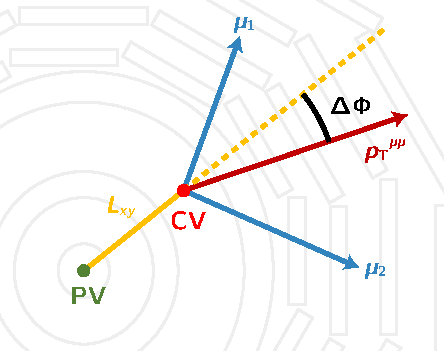
\includegraphics[width=.7\textwidth]{figures/displaced/LxyDef.pdf}
  \caption{Diagram of the key variables used in this analysis. A long-lived particle is produced at the primary vertex (PV) and travels some distance in the detector before decaying into two muons ($\Pgm_1$ and $\Pgm_2$), forming a common vertex (CV). The distance between these two vertices in the transverse plane is referred to as \Lxy, the transverse decay length. The angle between the \Lxy vector and the \pT vector of the dimuon system is referred to as $|\DeltaPhi|$, the collinearity angle in the transverse plane.}
  \label{fig:dd:keyvars}
\end{figure}

A common vertex fit of good quality results in a relatively small internal \Lxy uncertainty (\LxyErr), suggesting that the two muon tracks are consistent with originating from a common vertex.
The quantity $\Lxy/\LxyErr$ is referred as the \Lxy significance.
For a well-reconstructed dimuon corresponding to a long-lived particle decaying a few tens of centimeters away from the PV, as in signal events, this quantity is large.
On the other hand, background events from reconstruction mistakes or promptly produced particles are expected to result in dimuons with small \Lxy significance.
A large \Lxy significance is therefore a strong indicator of consistency with the long-lived particle hypothesis.

The collinearity angle in the transverse plane between the dimuon \pT vector ($\pT^{\Pgm\Pgm}$) and the \Lxy vector is referred to as $|\DeltaPhi|$.
For a real pair of muons originating from a CV formed from the decay of a long-lived particle originating at the PV, the resulting dimuon momentum vector points towards the PV, and $|\DeltaPhi|$ is small.
On the other hand, in most types of background events, this quantity is expected to be symmetric around $\pi/2$.
A small $|\DeltaPhi|$ is therefore a strong indicator of consistency with the long-lived particle hypothesis.

\Fig~\ref{fig:dd:keyvars} illlustrates these important quantities and their relationship to each other.

\section{Muon Reconstruction}
This analysis is a generic search for pairs of muons consistent with originating from a common vertex that is displaced with respect to the beamspot.
Such dimuon vertices can arise from decays of exotic long-lived particles, which are produced promptly (as a direct result of the hard interaction process and produced close to the beamspot) and travel for some distance before decaying.
As mentioned in \Sec~\ref{sec:dd:Trigger}, muons produced from such decays may not point towards the beamspot.
Most algorithms performing the offline reconstruction of muon tracks, however, include the beamspot; these reconstructions are described as being ``updated at the vertex.''
A search for displaced dimuons must therefore use a reconstruction algorithm that does not suffer from this beamspot constraint.

Muons reconstructed using only hits in the muon system are known as standalone muons.
Standalone muons are independent of the more precise information from the silicon tracker, and so have poorer spatial and momentum resolution than muons reconstructed using the tracker.
However, the reconstruction efficiency for tracker tracks with transverse impact parameter $d_0$ (the closest distance between the track and the beamspot in the transverse plane) of more than a few tens of \cm is essentially zero, while the muon system gives non-vanishing reconstruction efficiency even a few meters away from the beamspot.
Therefore, standalone muons are the reconstructed object of choice for a displaced dimuon search sensitive to longer lifetimes.
Furthermore, standalone muon reconstruction is available with and without the beamspot constraint.
Standalone muons without this beamspot constraint are the starting point for choosing a muon reconstruction suitable for studying displaced dimuons.

The analyses performed using Run~1 data used refitted standalone muons (RSA muons) as their primary muon reconstruction \cite{CMS-PAS-EXO-14-012,CMS-AN-14-176}.
Compared to ordinary standalone muons without the beamspot constraint, the RSA muon algorithm computes a final refit (an additional iteration in the standalone muon trajectory builder) excluding the beamspot.
This reconstruction was intended to reduce the inherent bias towards the beamspot exhibited by the standard standlone muon reconstruction designed to study muons originating directly from the \pp collision.
RSA muons thus have improved $d_0$ and \pT resolution compared to standalone muons.

Another muon reconstruction algorithm is the displaced standalone muon (DSA muon) reconstruction.
Compared to ordinary standalone muons without the beamspot constraint, the DSA muon reconstruction is seeded with groups of segments in the muon chambers with criteria similar to those used for the reconstruction of cosmic muons, as opposed to seeds used for the reconstruction of muons originating from \pp collisions \cite{CMS-DP-2015-015}.
This reconstruction was intended to further improve the \pT resolution of muons produced from highly displaced decays.

\Fig~\ref{fig:dd:REFF} shows graphs of the efficiency as a function of generated \Lxy to reconstruct a generated muon as DSA or as RSA, with and without the trigger applied, with respect to \mbox{$\PHiggs\to2\PLLP\to2\Pgm$} signal events in which both generated muons are within a detector acceptance, defined as
\begin{itemize}
  \item both generated muon $\pT > 25\GeV$
  \item both generated muon $|\eta| < 2$
  \item generated \mbox{$\Lxy < 500\cm$}
\end{itemize}
In order to observe sufficient statistics, all 33 of the \twoMu signal samples were combined together for these graphs.
The reconstruction efficiency decreases steadily as a function of generated \Lxy, dropping off sharply at about 600\cm, corresponding roughly to the start of the third barrel muon station, and the DSA reconstruction is consistently higher than the RSA reconstruction.
With the trigger applied, the reconstruction efficiency is high for both DSA and RSA muons, up until about 300\cm at which point the trigger efficiency seriously limits the number of passing events.

\Fig~\ref{fig:dd:PTRES_DSA_RSA} shows distributions of the \pT resolution for the DSA and RSA reconstructions, normalized to unit area, for generated events within acceptance, with and without the trigger applied, for the \twoMu signal sample with \FullSP{1000}{350}{350}.
The RSA reconstruction gives a visibly worse \pT resolution, with a larger ``shoulder'' near $-1$, indicating that RSA muons tend to underestimate the muon \pT compared to DSA muons.

\Figs~\ref{fig:dd:REFF}--\ref{fig:dd:PTRES_DSA_RSA} show that DSA muons have both a higher reconstruction efficiency and an improved \pT resolution over RSA muons.
The analysis presented in this thesis therefore primarily uses DSA muons.

\begin{figure}[htpb]
  \centering
  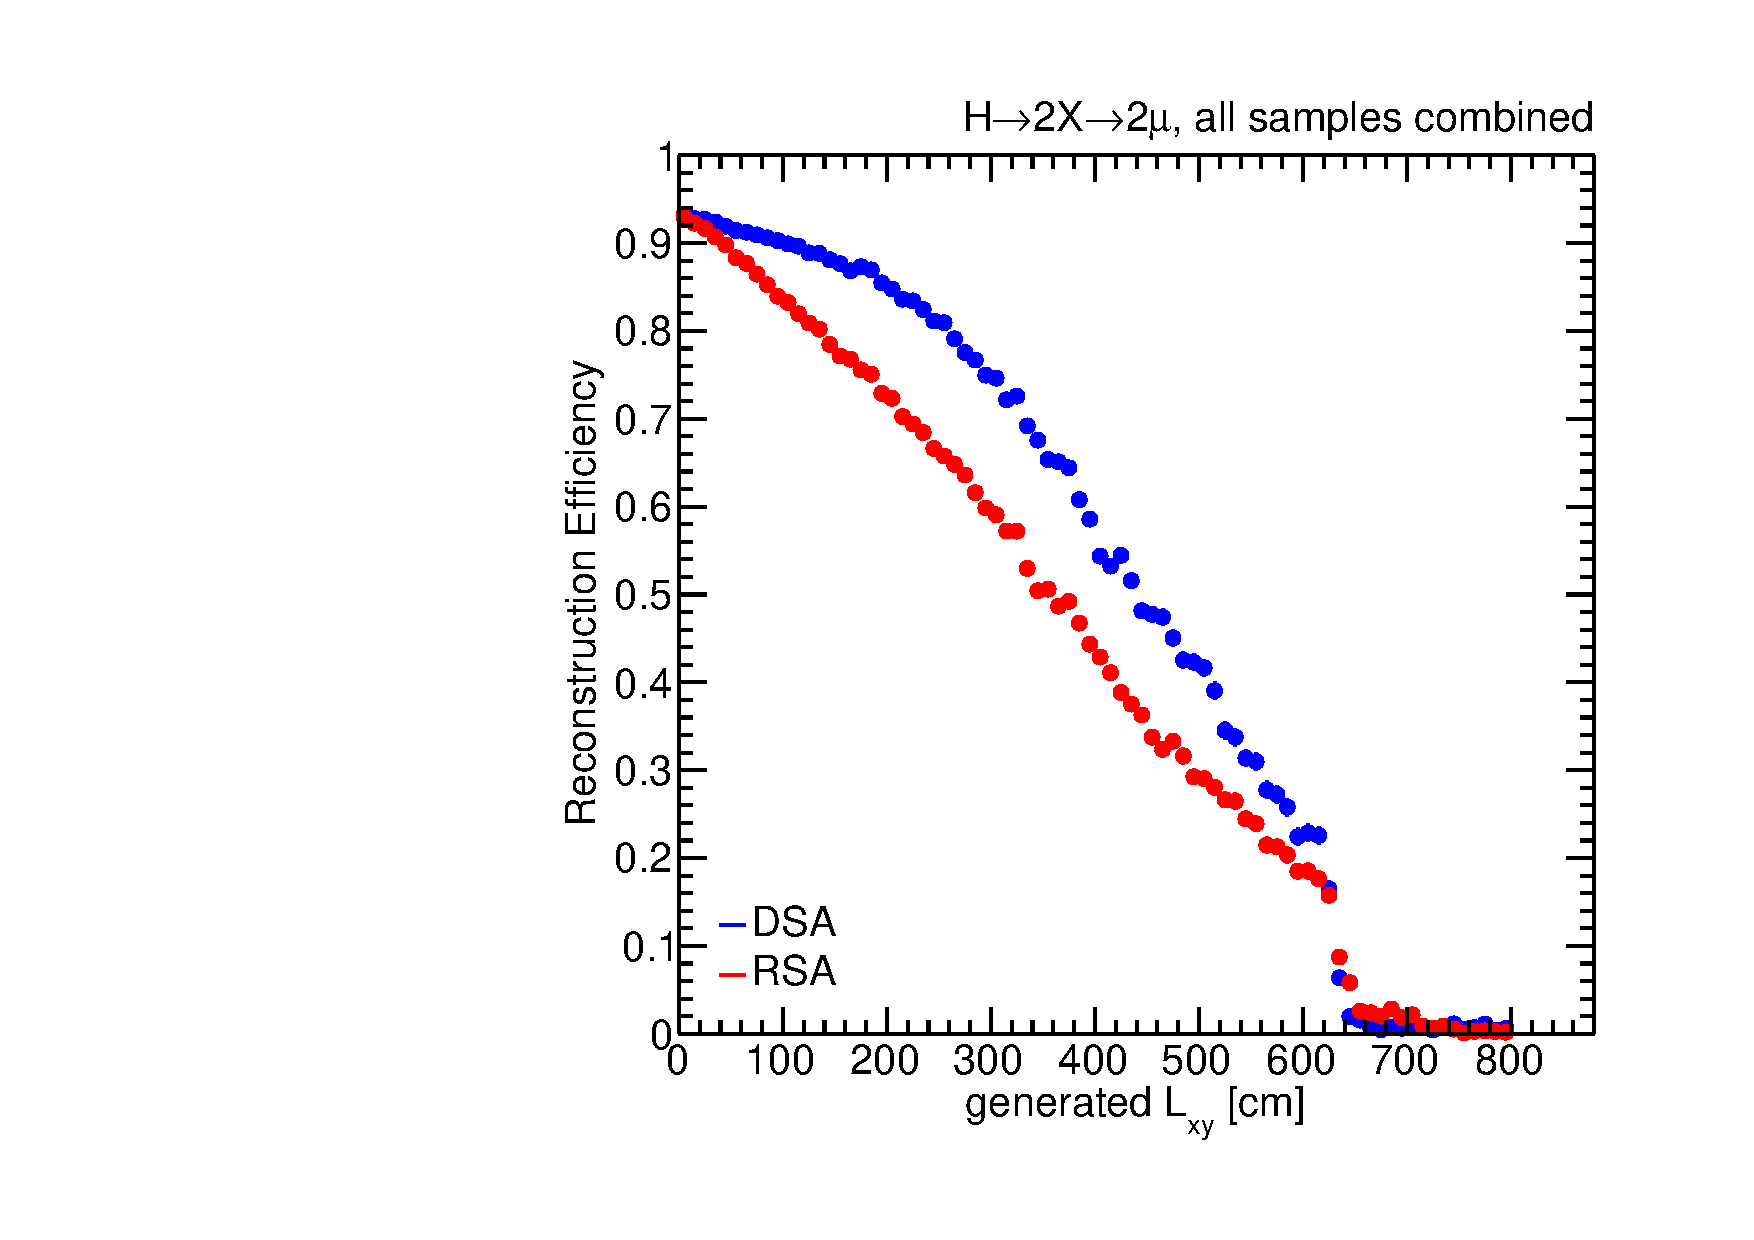
\includegraphics[width=\DSquareWidth]{figures/displaced/REFF_Lxy_2Mu2J_Global.pdf}
  \hspace*{-2em}
  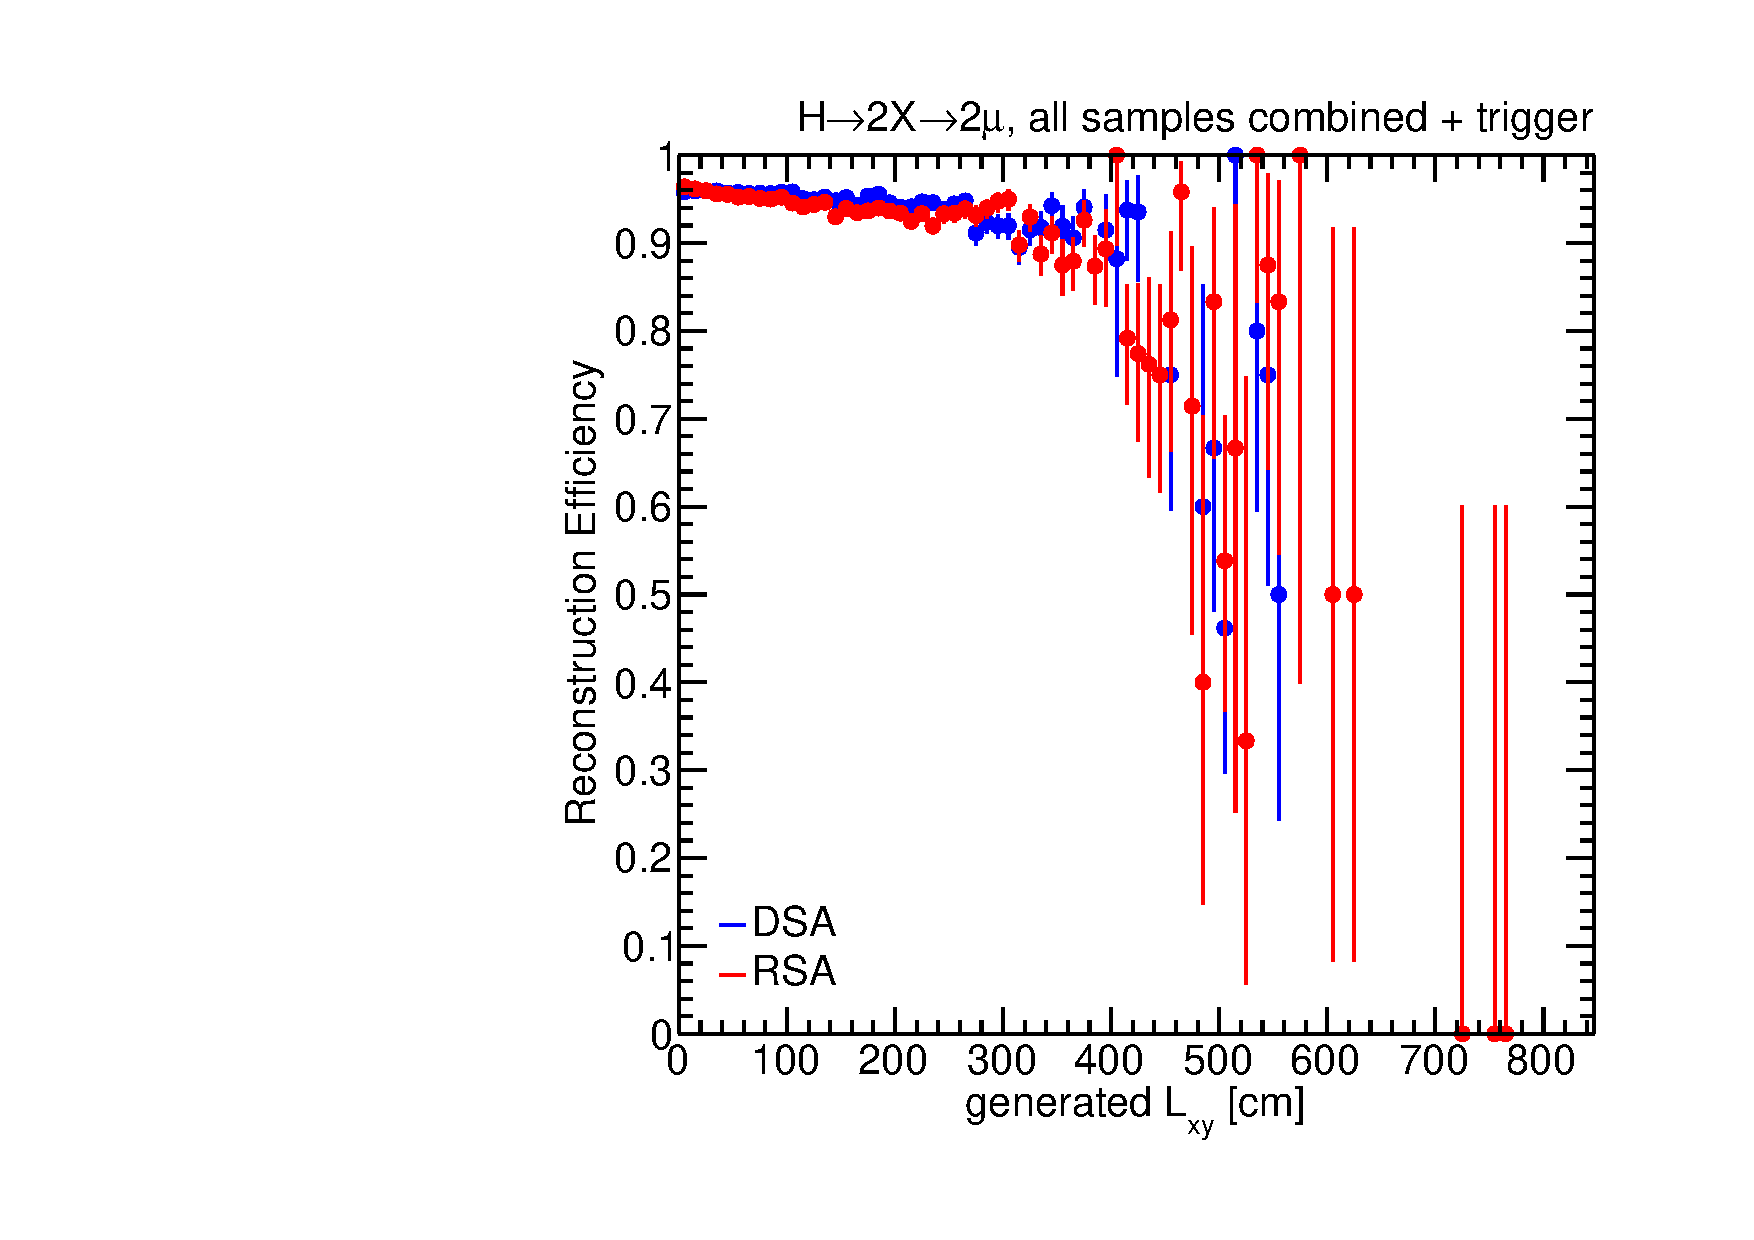
\includegraphics[width=\DSquareWidth]{figures/displaced/REFF_Lxy_Trig_2Mu2J_Global.pdf}
  \caption{DSA and RSA reconstruction efficiency as a function of generated \Lxy for \twoMu signal events combining all 33 signal samples, with respect to events within acceptance, (left) without and (right) with the trigger applied. Error bars are for statistical uncertainty only.}
  \label{fig:dd:REFF}
\end{figure}
\begin{figure}[htpb]
  \centering
  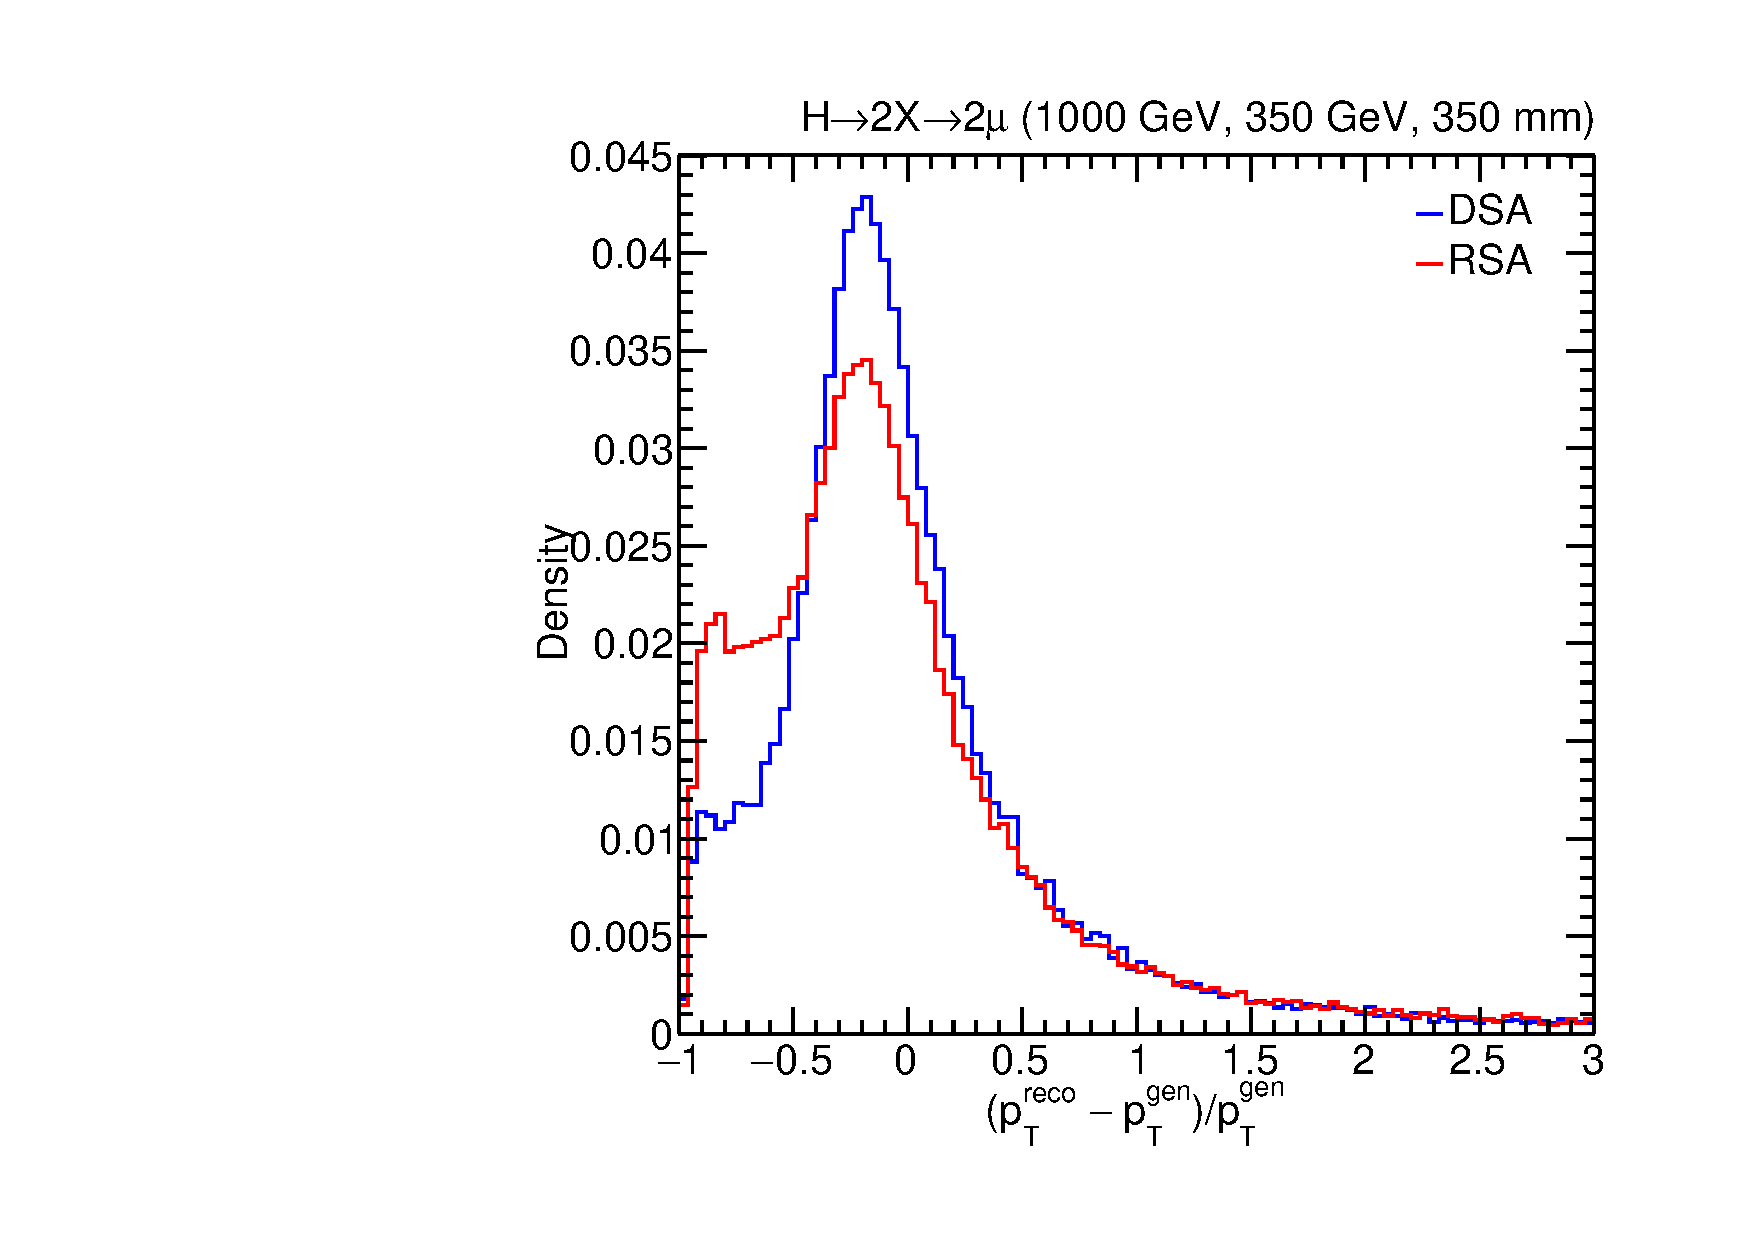
\includegraphics[width=\DSquareWidth]{figures/displaced/PTRES_2Mu2J_1000_350_350.pdf}
  \hspace*{-2em}
  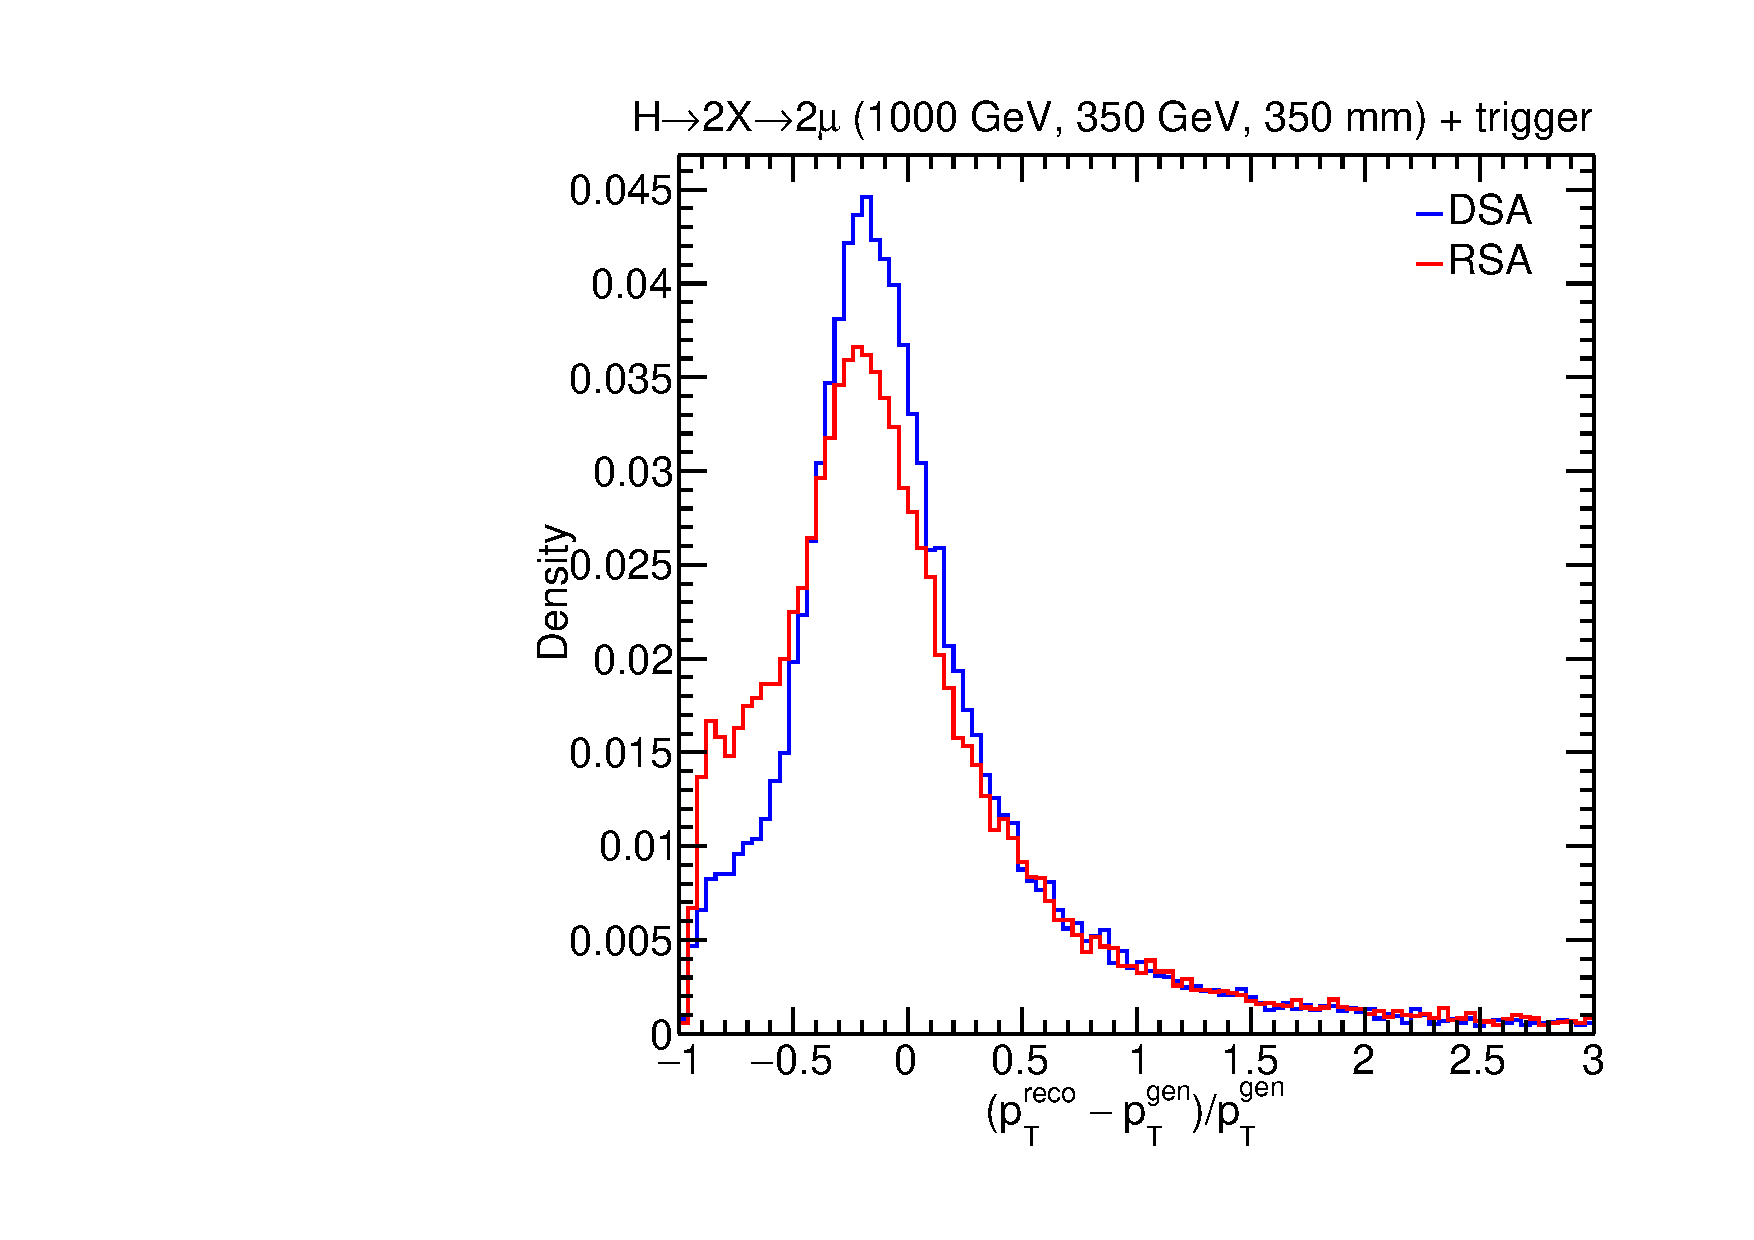
\includegraphics[width=\DSquareWidth]{figures/displaced/PTRES_Trig_2Mu2J_1000_350_350.pdf}
  \caption{DSA and RSA \pT resolution for generated events within acceptance, (left) without the trigger applied and (right) with the trigger applied, for the \twoMu signal sample with \FullSP{1000}{350}{350}.}
  \label{fig:dd:PTRES_DSA_RSA}
\end{figure}

\section{Event and Object Selection}
\subsection{Overview}
\label{sec:dd:GeneralStrategy}
An overview of the general strategy for selecting reconstructed events and objects consistent with displaced dimuons is as follows.
\clearpage
\begin{enumerate}
  \item \textbf{DSA muon preselection}. Begin with DSA muons as seeds for searching for displaced dimuons and apply a set of quality criteria to select muons that are reasonably well reconstructed. (\Sec~\ref{sec:dd:DSAQuality})
  \item \textbf{HLT-RECO matching}. Keep only events which contain offline reconstructed muons that match the online trigger muons passing the HLT. (\Sec~\ref{sec:dd:HLTMatching})
  \item \textbf{\DSAToPAT muon association}. Attempt to associate DSA muons with global or arbitrated tracker muons (referred to as PAT muons, named after the \textbf{P}hysics \textbf{A}nalysis \textbf{T}ools in the CMS software that processes them), and if they can be, replace the DSA muons with the associated PAT muons. This analysis focuses on the DSA muons that were \emph{not} associated with PAT muons, so this step essentially rejects DSA muons that are consistent with muons reconstructed using the tracker. (\Sec~\ref{sec:dd:Association})
  \item \textbf{DSA muon object selection}. Apply additional selections to remaining DSA muons that identify DSA muons in signal-like events and ensure that they are of good quality. (\Sec~\ref{sec:dd:DSAObject})
  \item \textbf{Dimuon formation from common vertex fit}. Form dimuons by fitting two DSA muon tracks to a common vertex. (\Sec~\ref{sec:dd:DimVertex})
  \item \textbf{Pairing criteria}. Select the 1--2 dimuons most likely to be signal dimuons according to a set of muon pairing criteria. (\Sec~\ref{sec:dd:PC})
  \item \textbf{Dimuon object selection}. Apply additional selections to dimuons that identify dimuons in signal-like events and ensure they are of good quality. (\Sec~\ref{sec:dd:DimuonObject})
  \item \textbf{Dimuon signal selection}. Apply additional selections to dimuons that require the dimuon be displaced from the beamspot and have a form consistent with the signal hypothesis that the dimuon originates from the decay of a long-lived particle into two oppositely-charged muons. (\Sec~\ref{sec:dd:DimuonSignal})
  \item \textbf{Cosmic muon suppression}. Apply additional requirements to suppress background events from cosmic muons. (\Sec~\ref{sec:dd:CosmicCuts})
\end{enumerate}

\subsection{DSA Muon Preselection}
\label{sec:dd:DSAQuality}
Event and object preselection begins with DSA muons.
The HLT path described in \Sec~\ref{sec:dd:Trigger} reconstructs muons at \Ltwo using a procedure similar to that used to reconstruct muons as refitted standalone (RSA) muons at the offline reconstructed level.
However, as discussed in the previous section, DSA muons were chosen as the starting point over RSA muons for their improved \pT resolution and higher reconstruction efficiency.
DSA muons are required to satisfy the following quality criteria:
\begin{itemize}
  \item reconstructed with hits in at least two muon stations, \ie $$N(\text{CSC stations}) + N(\text{DT stations}) > 1$$
  \item reconstructed with at least 13 hits in the muon stations, \ie $$N(\text{CSC hits}) + N(\text{DT hits}) > 12$$
  \item relative \pT uncertainty of less than 100\%, \ie $$\pTErr/\pT < 1$$
\end{itemize}

These quality criteria ensure that the DSA muons have acceptable \pT resolution and charge assignment.
\Fig~\ref{fig:dd:QCUT_PTRES} shows distributions of the DSA muon \pT resolution for the \twoMu signal sample with \FullSP{1000}{350}{350} for events split up by the $N_\text{hits}$ cut and for events split up by the $\pTErr/\pT$ cut, each population normalized to unit area.
The events satisfying the cut have reasonable \pT resolution, while the events failing the cut have very poor \pT resolution.
\Fig~\ref{fig:dd:QCUT_QDIFF} shows distributions of the difference between reconstructed and generated charge for the same signal sample, for events split up by the $N_\text{hits}$ cut and for events split up by the $\pTErr/\pT$ cut, each population normalized to unit area.
The events satisfying the cut are assigned the correct charge in more than 90\% of events, while the events failing the cut are assigned the correct charge in only around 60\% of events.

\begin{figure}[htpb]
  \centering
  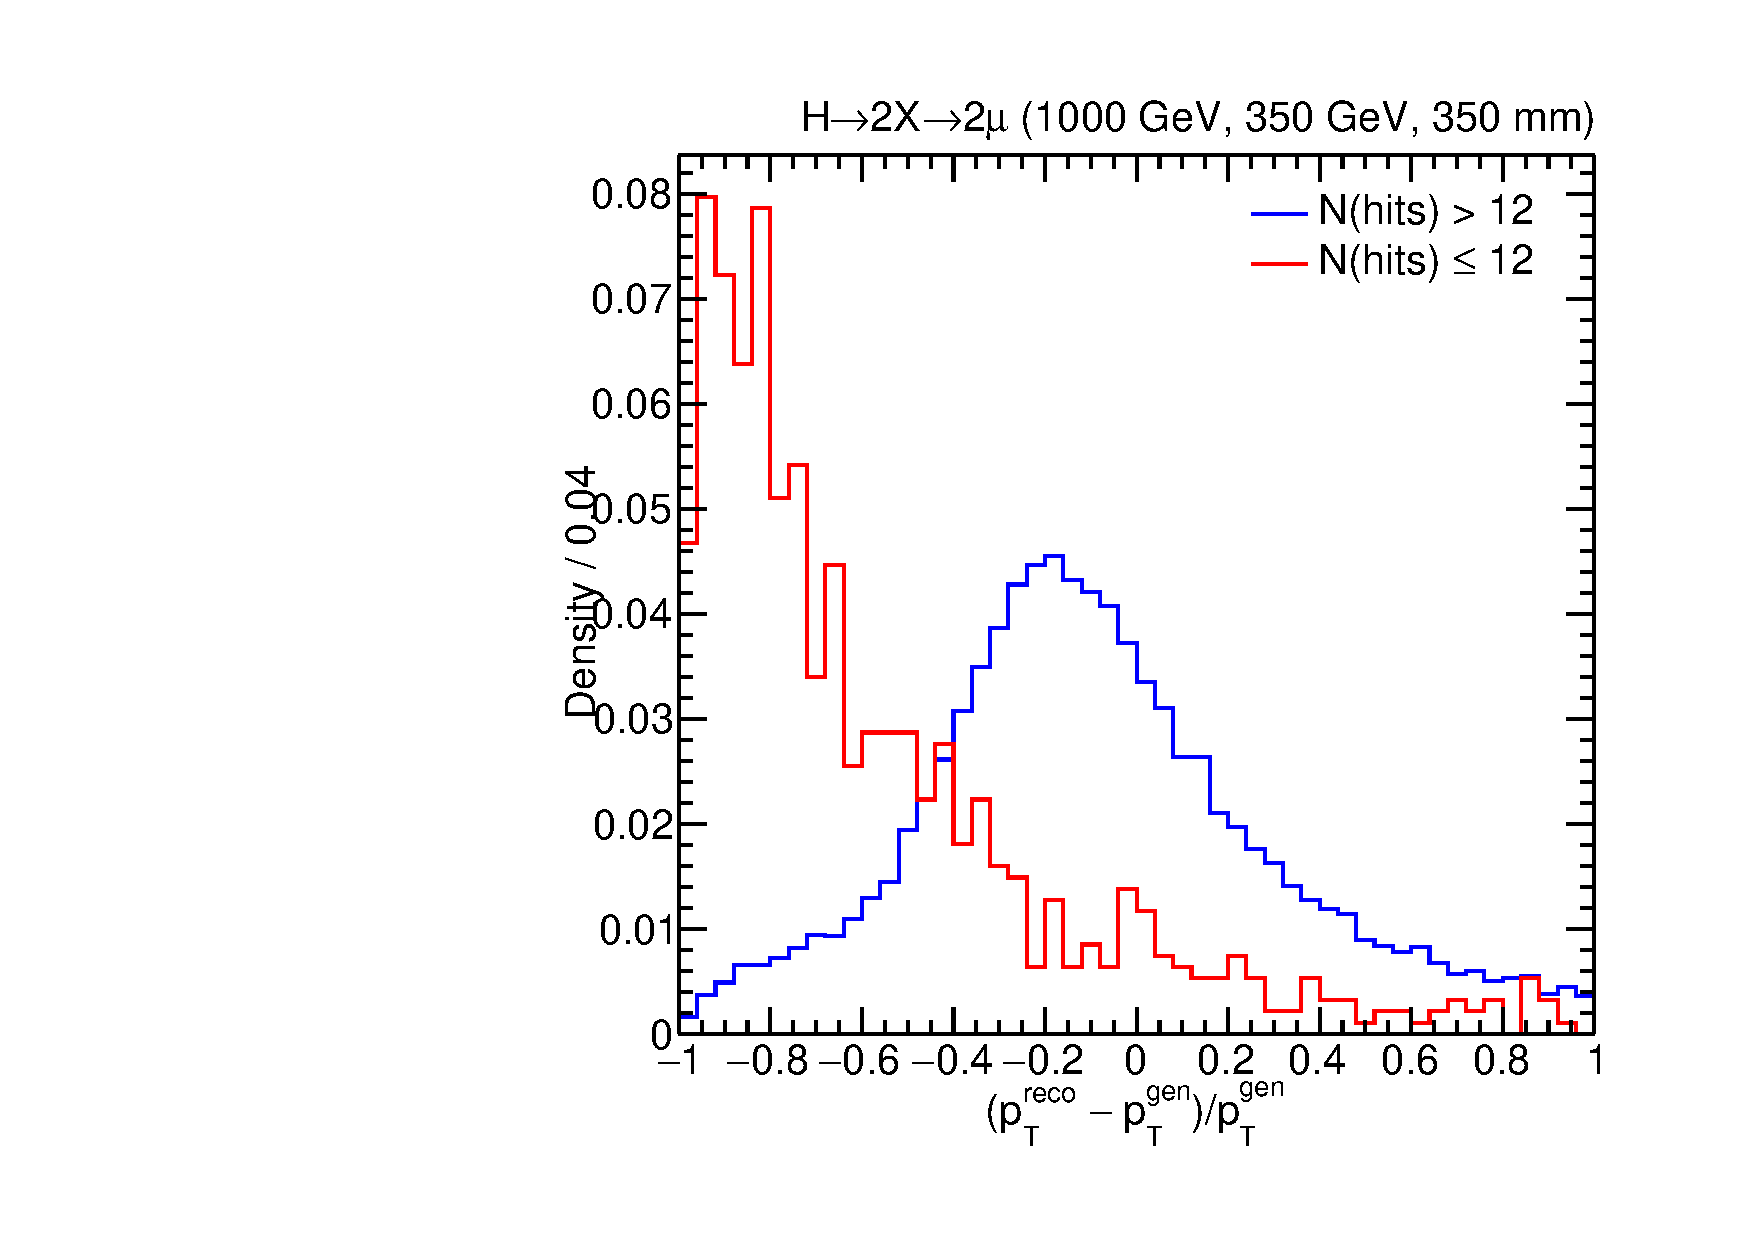
\includegraphics[width=\DSquareWidth]{figures/displaced/QCUTRES_Sig_pTRes_hits_1000_350_350.pdf}
  \hspace*{-2em}
  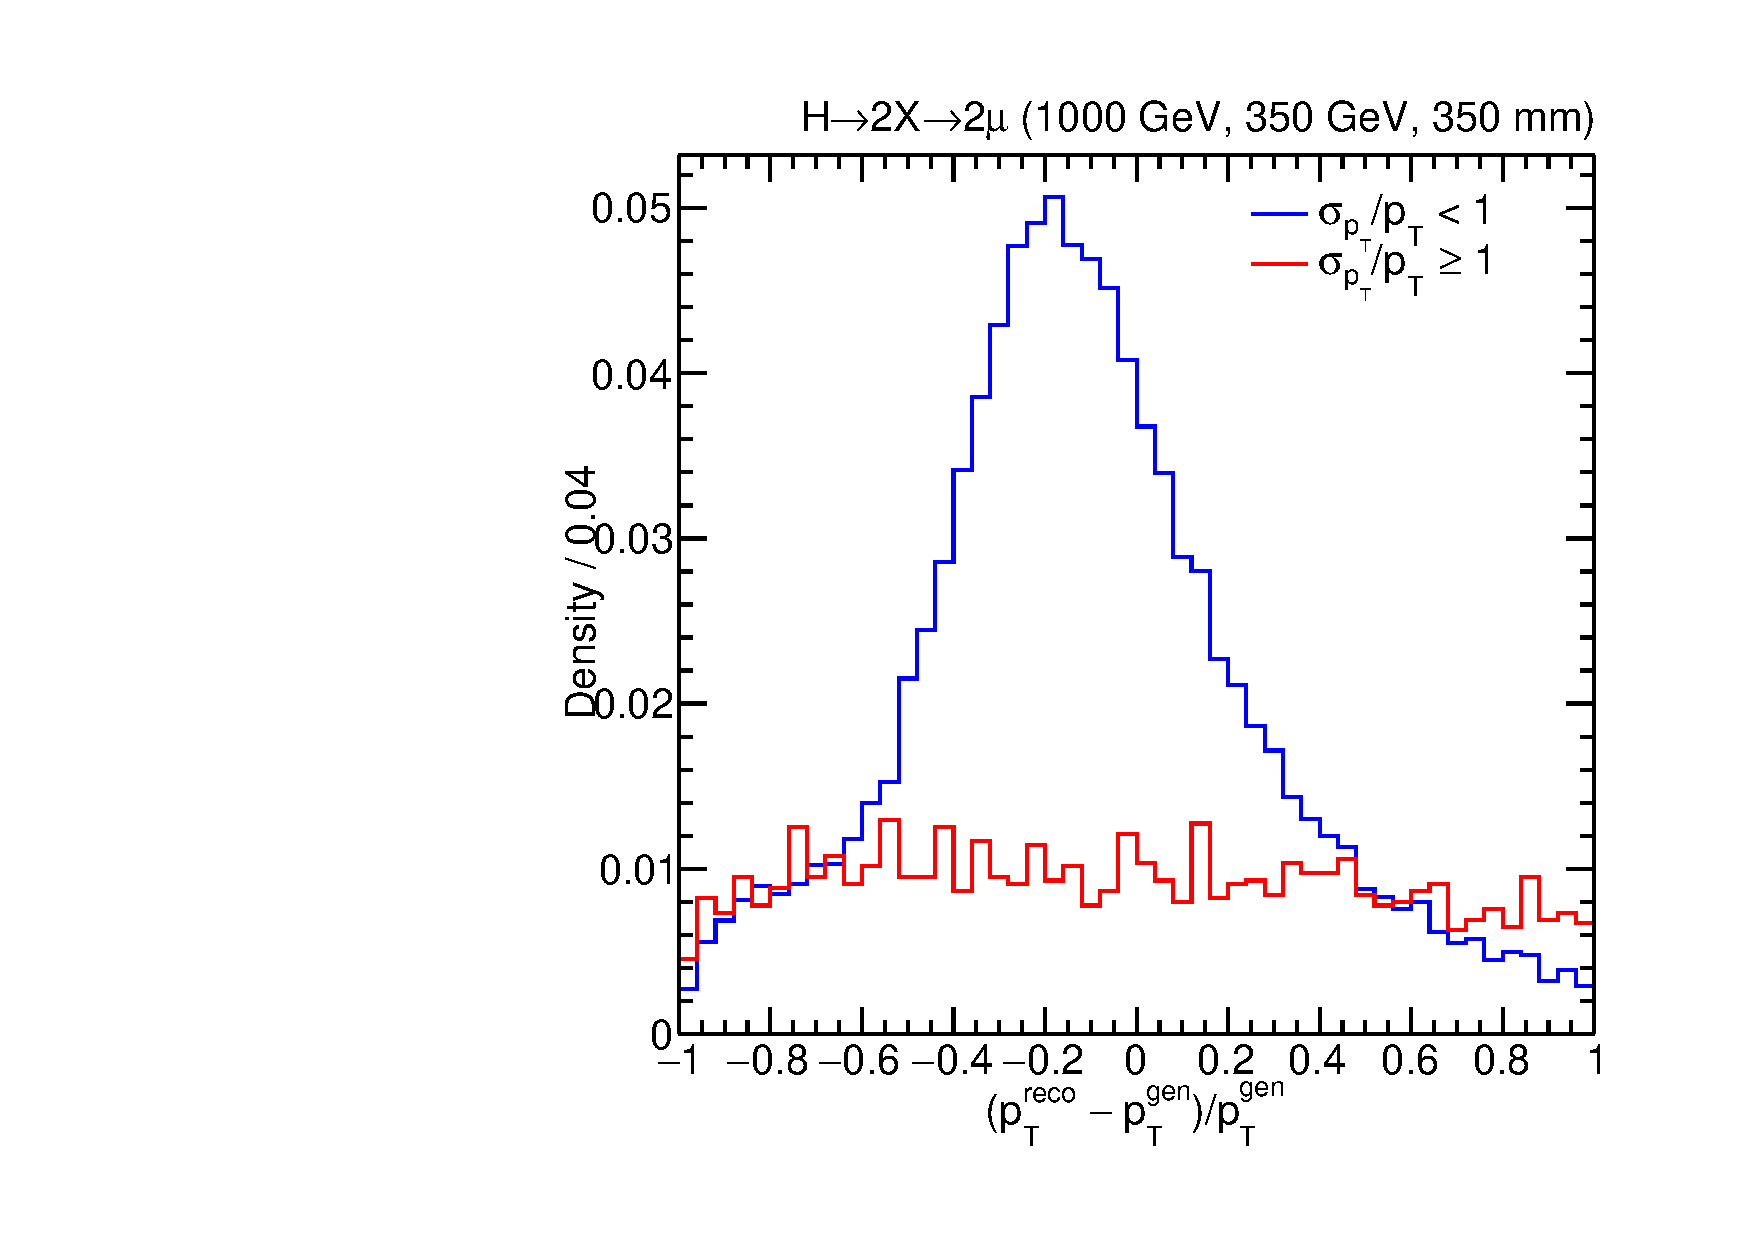
\includegraphics[width=\DSquareWidth]{figures/displaced/QCUTRES_Sig_pTRes_fpte_1000_350_350.pdf}
  \caption{DSA muon \pT resolution, normalized to unit area, for the \twoMu signal sample with \FullSP{1000}{350}{350} for (left) events with $N_\text{hits} > 12$ and $N_\text{hits} \leq 12$ separately, and (right) events with $\pTErr/\pT \geq 1$ and $\pTErr/\pT < 1$ separately.}
  \label{fig:dd:QCUT_PTRES}
\end{figure}
\begin{figure}[htpb]
  \centering
  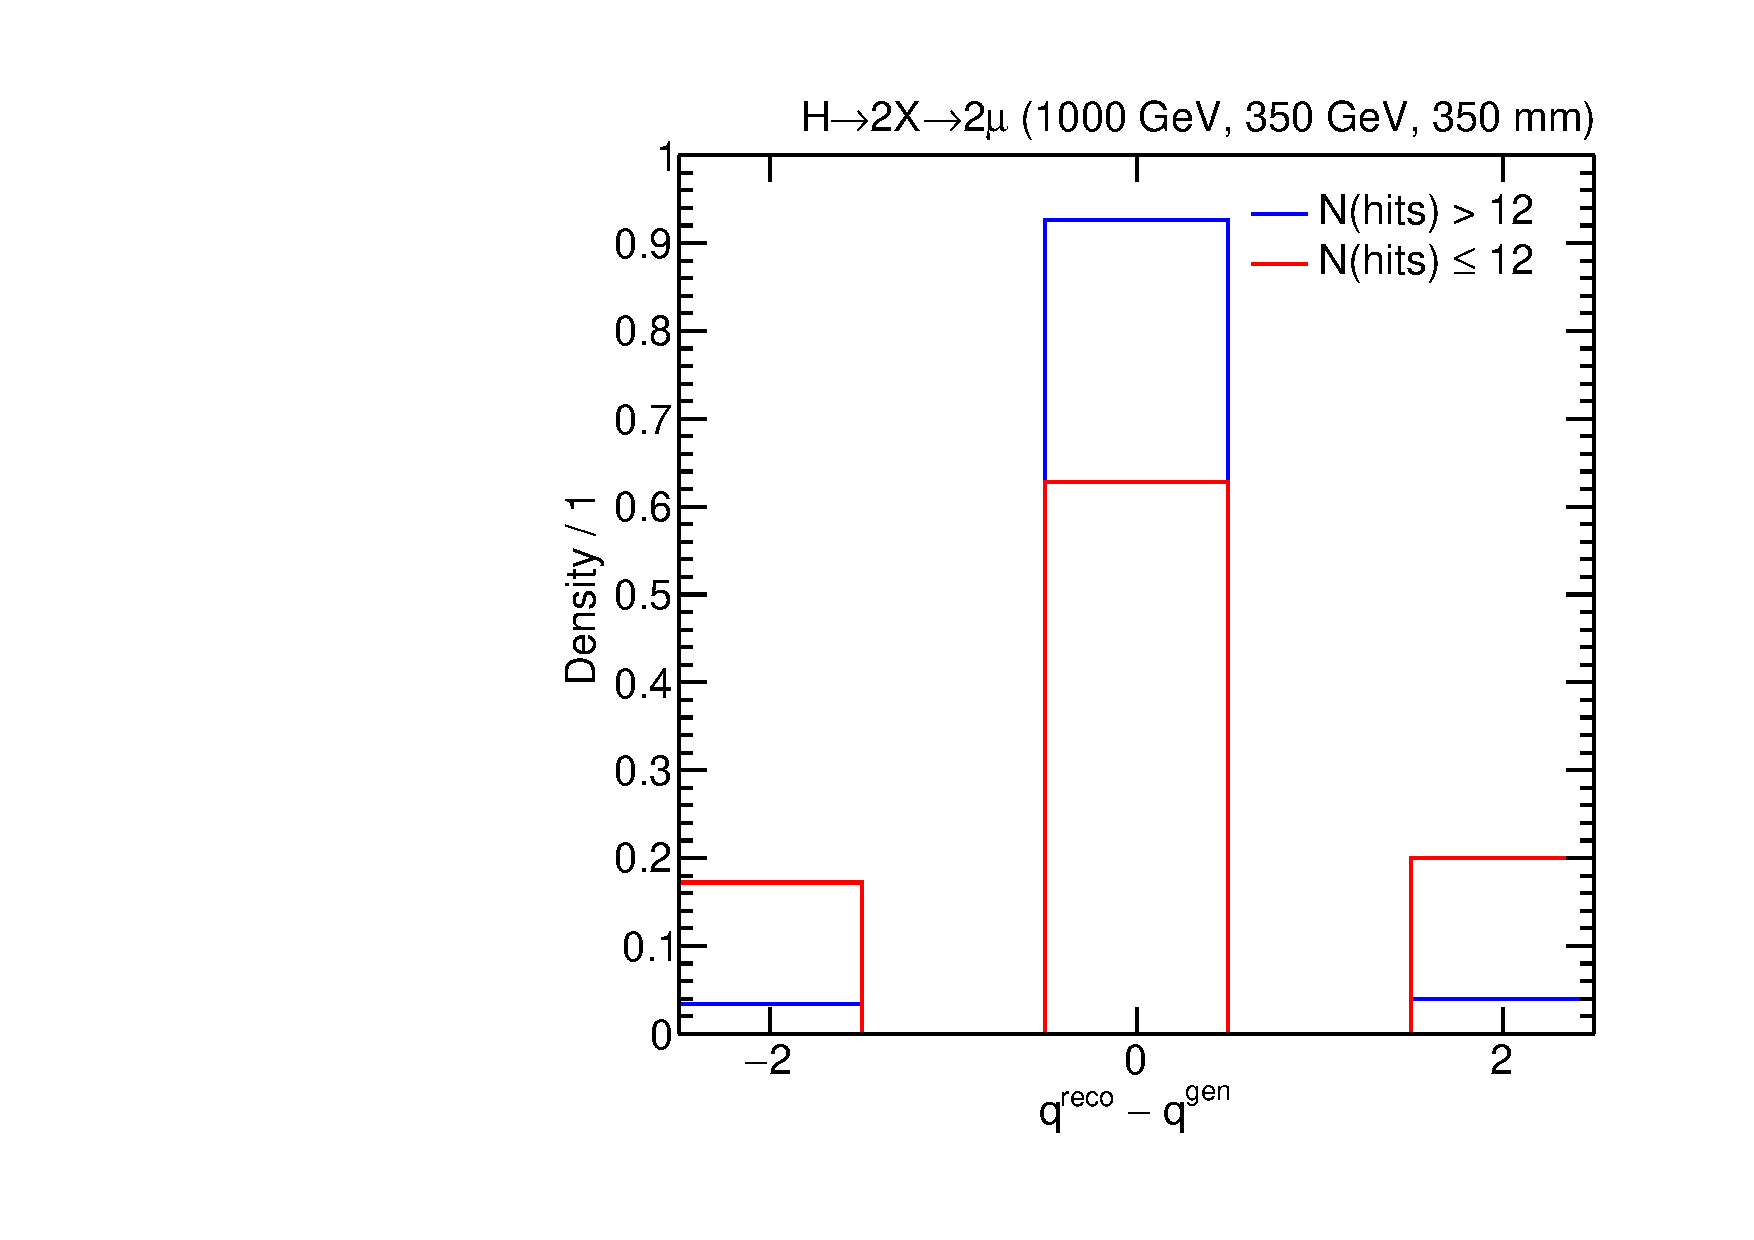
\includegraphics[width=\DSquareWidth]{figures/displaced/QCUTRES_Sig_qdiff_hits_1000_350_350.pdf}
  \hspace*{-2em}
  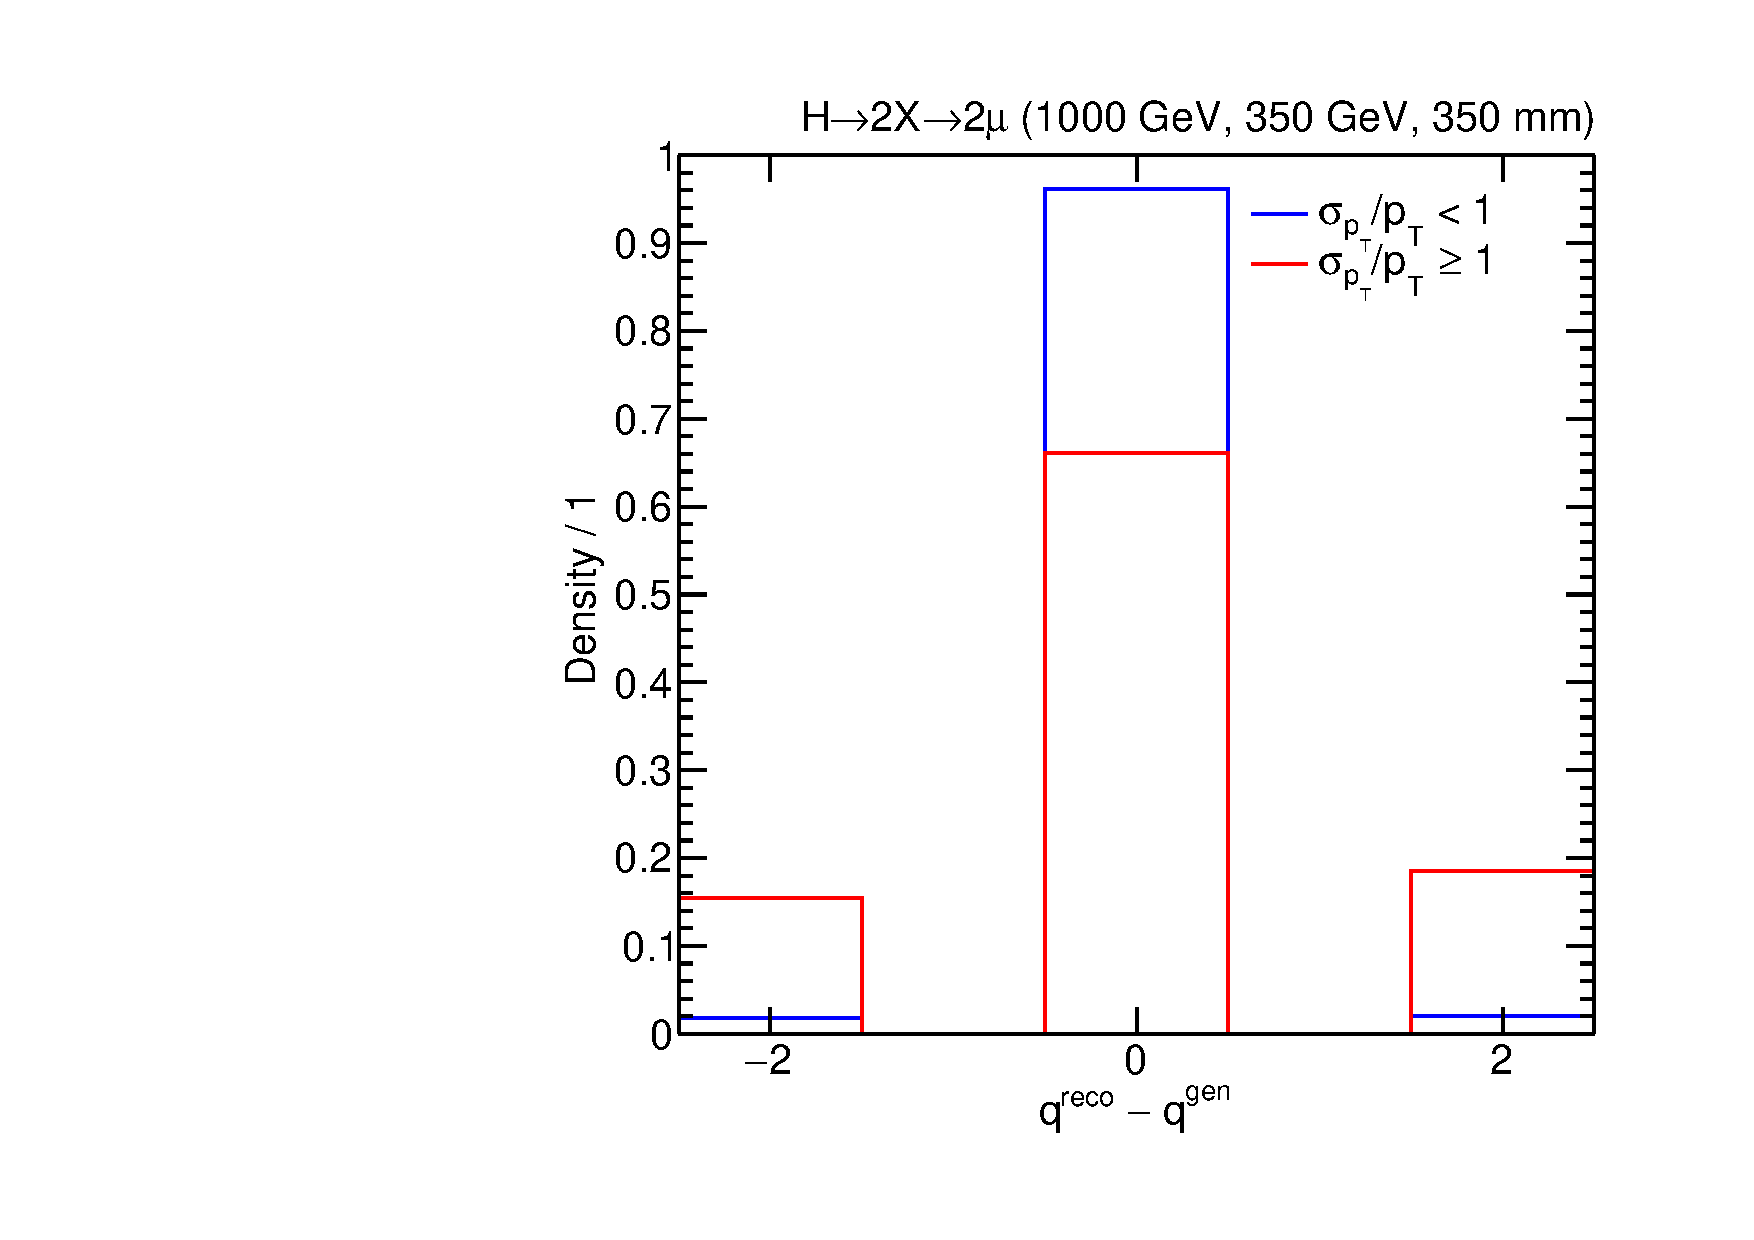
\includegraphics[width=\DSquareWidth]{figures/displaced/QCUTRES_Sig_qdiff_fpte_1000_350_350.pdf}
  \caption{DSA muon charge difference, normalized to unit area, for the \twoMu signal sample with \FullSP{1000}{350}{350} for (left) events with $N_\text{hits} > 12$ and $N_\text{hits} \leq 12$ separately, and (right) events with $\pTErr/\pT \geq 1$ and $\pTErr/\pT < 1$ separately.}
  \label{fig:dd:QCUT_QDIFF}
\end{figure}

\subsection{HLT-RECO Matching}
\label{sec:dd:HLTMatching}
Next, only events in which the HLT decision is matched using the preselected DSA muons are kept, in a procedure referred to as HLT-RECO matching.
This ensures that the quickly-reconstructed, coarser-resolution muons reconstructed by the trigger system have counterparts among muons reconstructed offline using the higher-precision data of the full event.
For the purposes of HLT-RECO matching, DSA muons are required to pass loose \pT and $\eta$ requirements: $\pT > 10\GeV$ and $|\eta| < 2.0$.
These DSA muons are referred to as DSA muons for trigger matching.
Let \deltaR refer to the angular proximity in $\eta$-$\phi$ space between two three-vectors, defined as
\begin{equation}
  \Delta R = \sqrt{\left(\Delta\eta\right)^2 + \left(\Delta\phi\right)^2}
  \label{eq:dd:deltaR}
\end{equation}
Then HLT-RECO matching requires that each of the pair of distinct DSA muons for trigger matching lie within cones of $\deltaR < 0.4$ around each muon among pairs of muons reconstructed at \Ltwo passing the trigger (HLT muons).

The \pT, $\eta$, and \deltaR requirements were all chosen to empirically optimize the tradeoff between efficiency and purity, matching as many events as possible while keeping the frequency of accidental matches to poor quality muons low.
The HLT-RECO matching procedure retains more than 98\% of \twoMu signal events that passed the trigger and have at least two DSA muons for trigger matching.

The HLT-RECO matching requirement ensures, at the event level, that the trigger decision is confirmed using objects reconstructed offline.
The subsequent object selection, however, does not require that selected dimuons be formed from pairs of triggering HLT muons.
This allows the analysis to be sensitive to \fourMu final states, in which two of the four muons passed the trigger, but all four muons are signal muons.

\subsection{\DSAToPAT Muon Association}
\label{sec:dd:Association}
This analysis begins with DSA muons to identify potential displaced muon events, specifically focusing on highly displaced events in which the long-lived particle travels far enough before decaying that a track is not observed in the tracker.
Implementing this requirement necessitates development of a procedure to efficiently associate DSA muons to muons reconstructed using the tracker.
This association improves not only potential signal discrimination, but also background rejection.
Ensuring that this procedure is both highly efficient (\ie muons that should be associated, are) and highly pure (\ie muons that should not be associated, are not) requires some care.
This section describes the details of the association procedure.

\subsubsection{PAT Muons and Matching Criteria}
Offline reconstructed muons having either of the following properties are considered:
\begin{itemize}
  \item \textbf{Global muons}. Global muons are muons reconstructed by association a tracker track with a standalone muon by collecting all the hits from both and performing a full track fit, called a global muon fit. Global muons are the primary muon reconstruction used by most CMS analyses.
  \item \textbf{Arbitrated tracker muons}. In order to deal with cases in which global muon reconstruction is inefficient, tracker muons were developed. Tracker muons do not require a standalone muon; instead, a tracker track is extrapolated and associated with hits in the muon system. In the case of multiple tracker tracks associated with the same muon hits, an algorithm called arbitration chooses which association to prefer such that no two tracker muons share muon segments; these tracker muons are referred to as arbitrated tracker muons.
\end{itemize}
The muons considered in this analysis that are reconstructed offline using both the tracker and the muon system are referred to as PAT muons.
(PAT is an abbreviation for \textbf{P}hysics \textbf{A}nalysis \textbf{T}ools, a toolkit that is part of the CMS software and which is used to process event and object reconstruction.)
A PAT muon may be both a global muon and an arbitrated tracker muon, and good quality PAT muons are often both.

Candidate PAT muons are associated to DSA muons when they satisfy one of two matching criteria, which are applied in different contexts in a procedure described below. The two matching criteria are
\begin{itemize}
  \item \textbf{Segment-matched}: A PAT muon is segment-matched to a DSA muon if the PAT muon shares all of its muon system segments with at least 2/3 of the muon system segments used to reconstruct the DSA muon. PAT muon segments and DSA muon segments are compared coordinate by coordinate for equality and are considered the same if their coordinates match.
  \item \textbf{Proximity-matched}: A PAT muon is proximity-matched to a DSA muon if the \deltaR between
    \begin{itemize}
      \item the position vector of the innermost hit of the DSA muon and
      \item the momentum vector of the PAT muon helically extrapolated (in the magnetic field) to the point of closest approach to the innermost hit of the DSA muon
    \end{itemize}
    is less than 0.4, with tighter requirements applied in the procedure described below.
\end{itemize}

The proximity match is defined as it is above because DSA muons are sometimes reconstructed with an incorrect $\eta$ coordinate, and would not pass a more standard angular proximity match between the momentum directions of the DSA and PAT muons.
The helical extrapolation and comparison between the position and momentum improved the efficiency of the proximity match.

\subsubsection{\DSAToPAT Association Procedure}
The general procedure is as follows: given a DSA muon, associate segment-matched PAT muons to the DSA muon, using additional criteria to disambiguate among multiple segment-matched PAT muons.
These additional disambiguation criteria include checking segment-matched PAT muons are also the PAT muon with the smallest proximity-match \deltaR (as defined above) and/or requiring that segment-matched muons be global and that they be reconstructed from hits in at least 7 tracker layers.
If no PAT muons segment-matched the DSA muon, the smallest-\deltaR proximity-matched PAT muon is associated to the DSA muon if its proximity-match \deltaR is sufficiently small: the threshold is 0.1 if the proximity-matched PAT muon is global only, and 0.15 if the proximity-matched PAT muon is arbitrated tracker (whether or not it is global).
The full technical details of the procedure are depicted in \Fig~\ref{fig:dd:repdiagram}.

\begin{figure}[p]
  \centering
  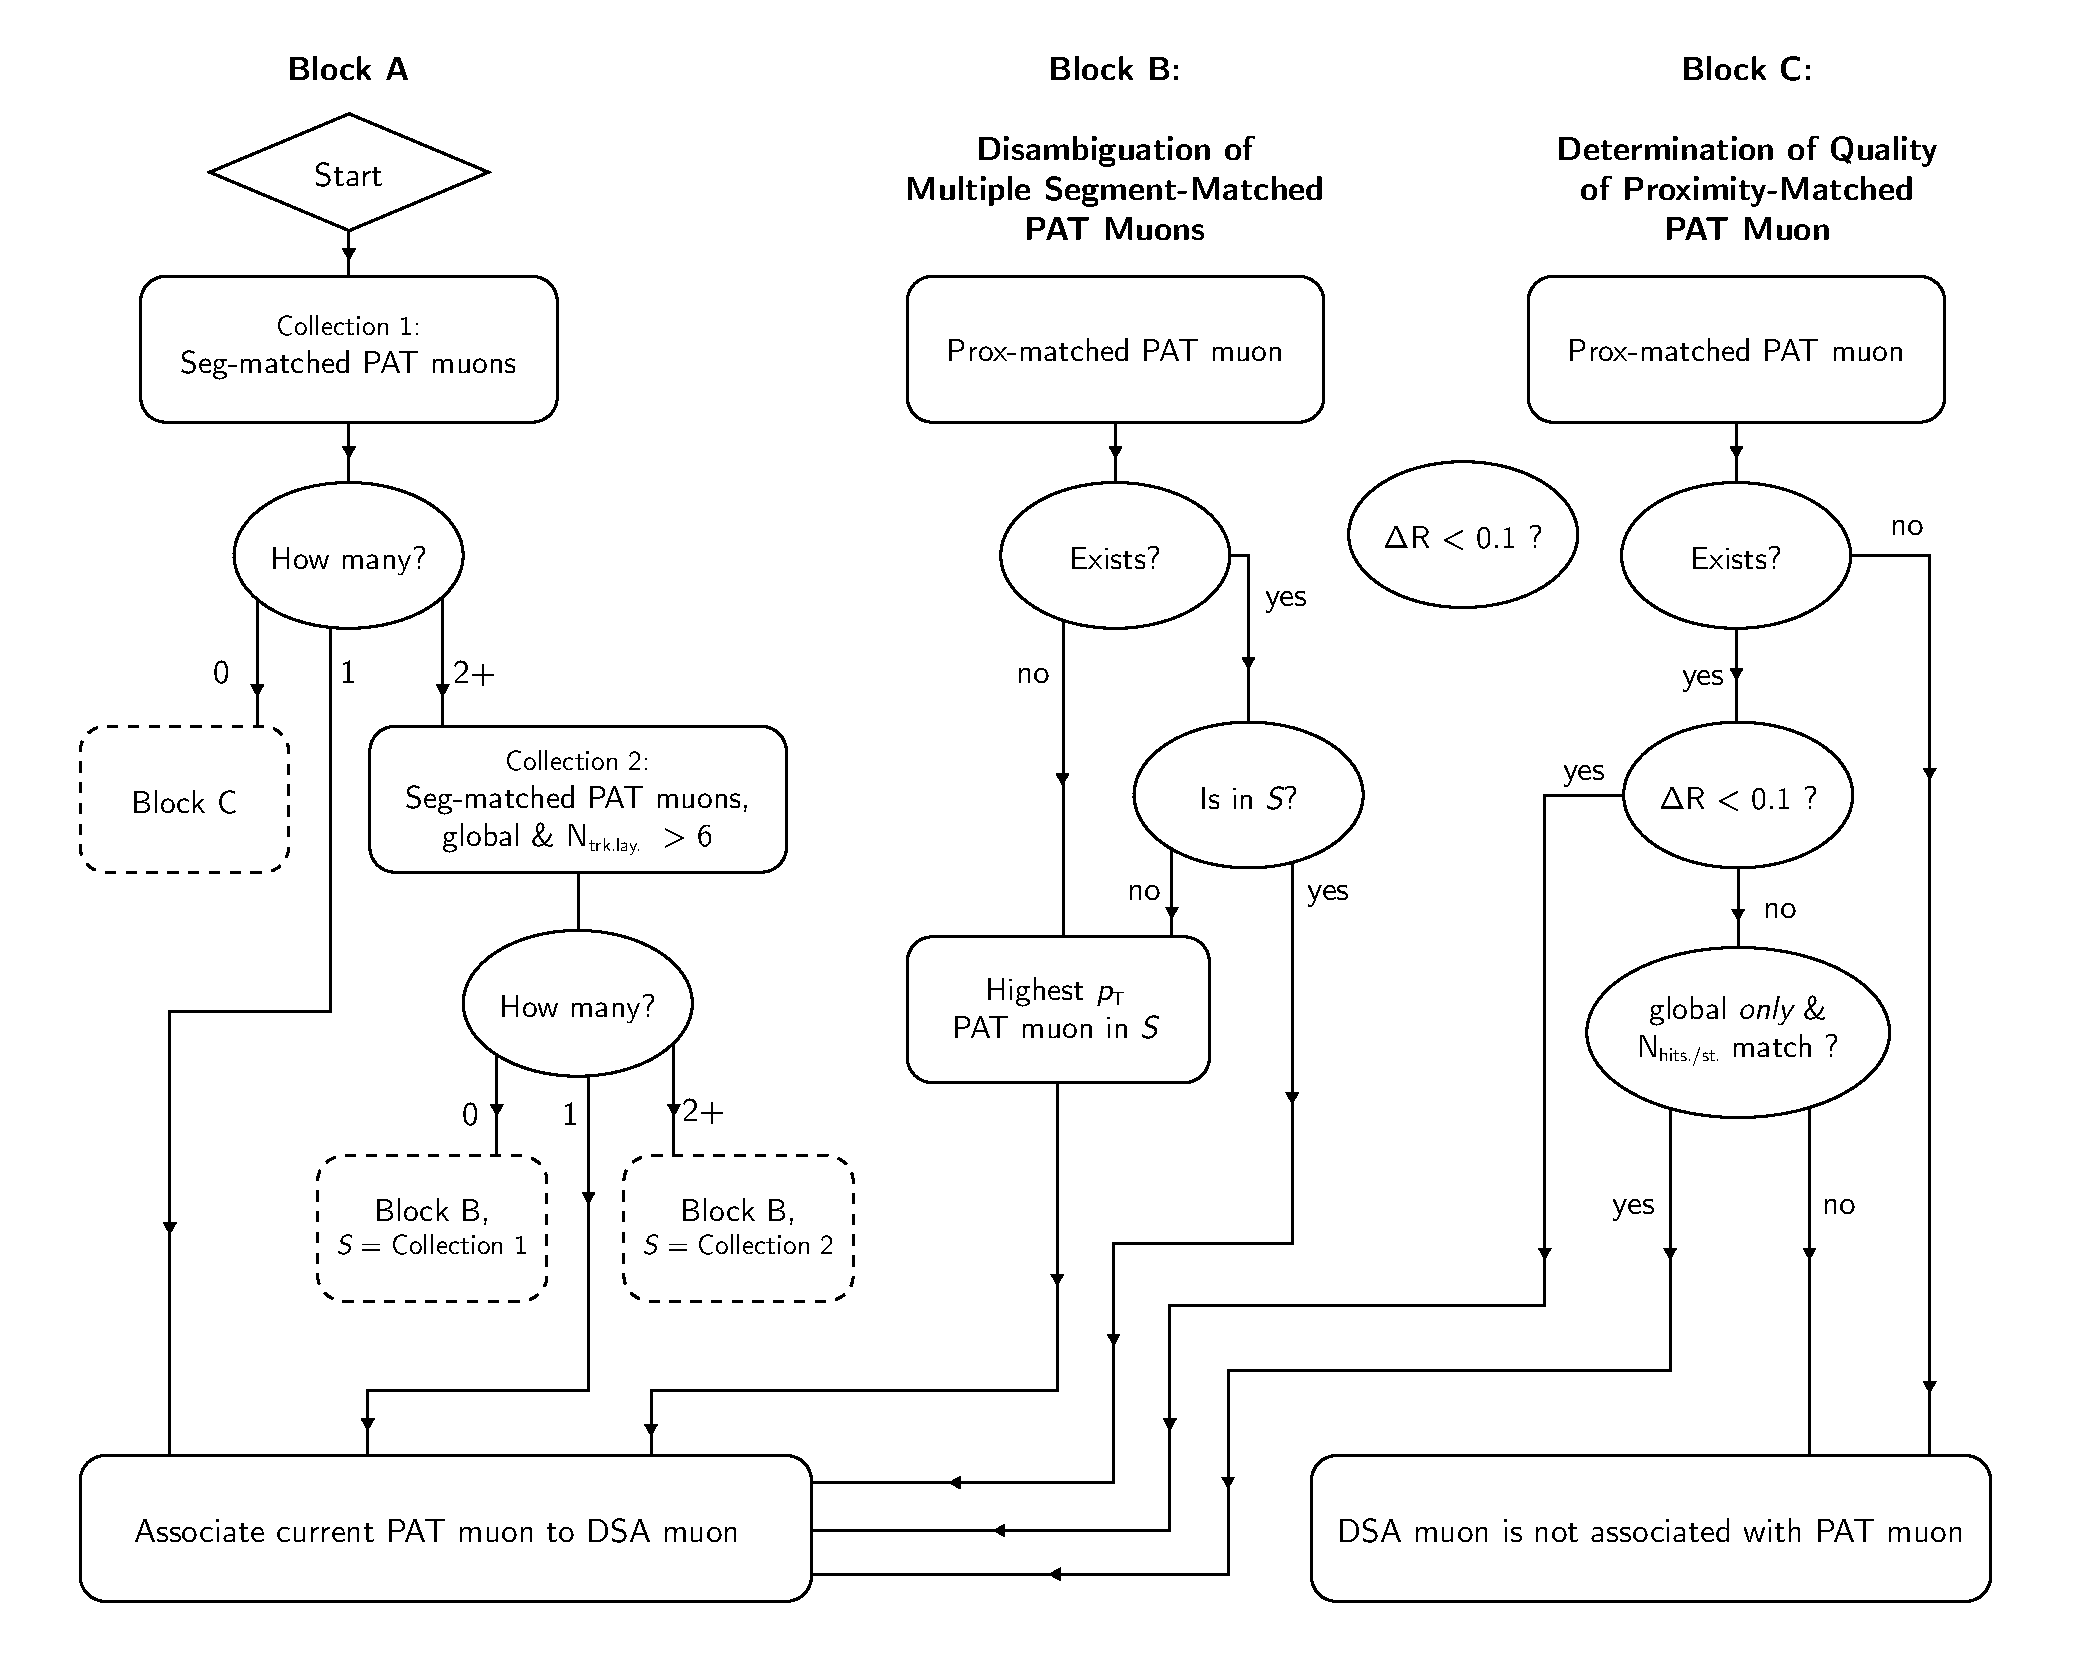
\includegraphics[width=\textwidth]{figures/displaced/ReplacementDiagram.pdf}
  \caption{Flowchart depicting the technical details of the \DSAToPAT association procedure. The procedure begins by considering segment-matched PAT muons. If there are multiple segment-matched PAT muons, then some temporary quality cuts are applied: the requirements that the muon be global and that it be reconstructed from at least 7 tracker layers (abbreviated $N_\text{trk. lay.}$). When there are multiple segment matches, the PAT muon that has the smallest proximity-match \deltaR is used to disambiguate between them, if possible. If there are no segment matches, then the proximity-matched PAT muon is taken as the match if its proximity \deltaR is sufficiently small, depending on whether the proximity-matched PAT muon is a tracker muon or only a global muon.}
  \label{fig:dd:repdiagram}
\end{figure}

This procedure prioritizes segment-matched PAT muons over proximity-matched PAT muons.
Several combinations of criteria were used to determine the quality selection used to disambiguate segment-matched PAT muons; the combination used here (global and number of tracker layers) was found to be optimal in terms of increasing the efficiency to match to the correct PAT muon.
In principle, there exists the case that a proximity-matched PAT muon does not exist or is not among the segment-matched PAT muons.
In this case, we were prepared to fall back to associating to the highest-\pT PAT muon among the collection of segment-matched PAT muons.
However, this situation never actually occurs in practice.

The \deltaR thresholds in the case that there were no segment-matched PAT muons were chosen empirically to increase the matching efficiency while keeping the rate of false, accidental matches low.
At the time of this writing, this analysis does not access the muon system segments used to reconstruct the standalone muons used to form global muons, and so a PAT muon that is global only cannot be segment-matched to a DSA muon.
This has little practical effect on the efficiency to correctly associate DSA muons to PAT muons in this analysis.
For the small fraction of PAT muons that are global only and should be associated with a DSA muon, the proximity-matched PAT muon is often the correct choice.
Therefore, the \deltaR threshold for global-only PAT muons was set at 0.1.
As missed matches can lead to a high rate of background events, this association procedure is also designed to be liberal: if a DSA muon can be reasonably associated with a PAT muon, it should be, even at the cost of a few accidental matches.
Therefore, in the case of no segment-matched PAT muons and a proximity-matched PAT muon that is a tracker muon, the procedure associates to the DSA muon the proximity-matched PAT muon if its proximity \deltaR is less than 0.15 as a final compromise between efficiency and purity.

As mentioned previously, the analysis presented in this thesis focuses only on the DSA muons that were not associated to PAT muons.
To this end, DSA muons are replaced with any associated PAT muons, and so the association step effectively functions as a rejection of DSA muons that can be associated to PAT muons.
The effect of this is that this analysis, using DSA muons, does not benefit from the improved resolution of PAT muons, but it benefits tremendously from the superior background rejection.
This is the analysis sensitive to the longest lifetimes, with long-lived particles decaying in the outer region of the tracker and outside the tracker through the muon system.

The PAT association procedure is very effective in suppressing \pp collision backgrounds, such as those modeled by the MC background samples.
\Figs~\ref{fig:dd:REPEFF_MC_LxySig}--\ref{fig:dd:REPEFF_MC_Lxy} are histograms of dimuon $\Lxy/\LxyErr$ and $\Lxy$ in MC background samples, with each process scaled to its equivalent luminosity as discussed in \Sec~\ref{sec:dd:EqLumi}, before and after the association procedure.
The PAT association suppresses events in MC background by a factor of $10^5$, reducing the number of dimuons from 12 million to 236.
For these histograms, a \pT cut of 10\GeV is applied to DSA muons on top of the preselection criteria.
This is a requirement that is part of the muon object selection (see \Sec~\ref{sec:dd:DSAObject}), but is applied here more clearly demonstrate the effect of the PAT association procedure by suppressing secondary, low-\pT muons not associated to PAT muons, such as those from other \pp collisions in the bunch crossing.

\begin{figure}[p]
  \centering
  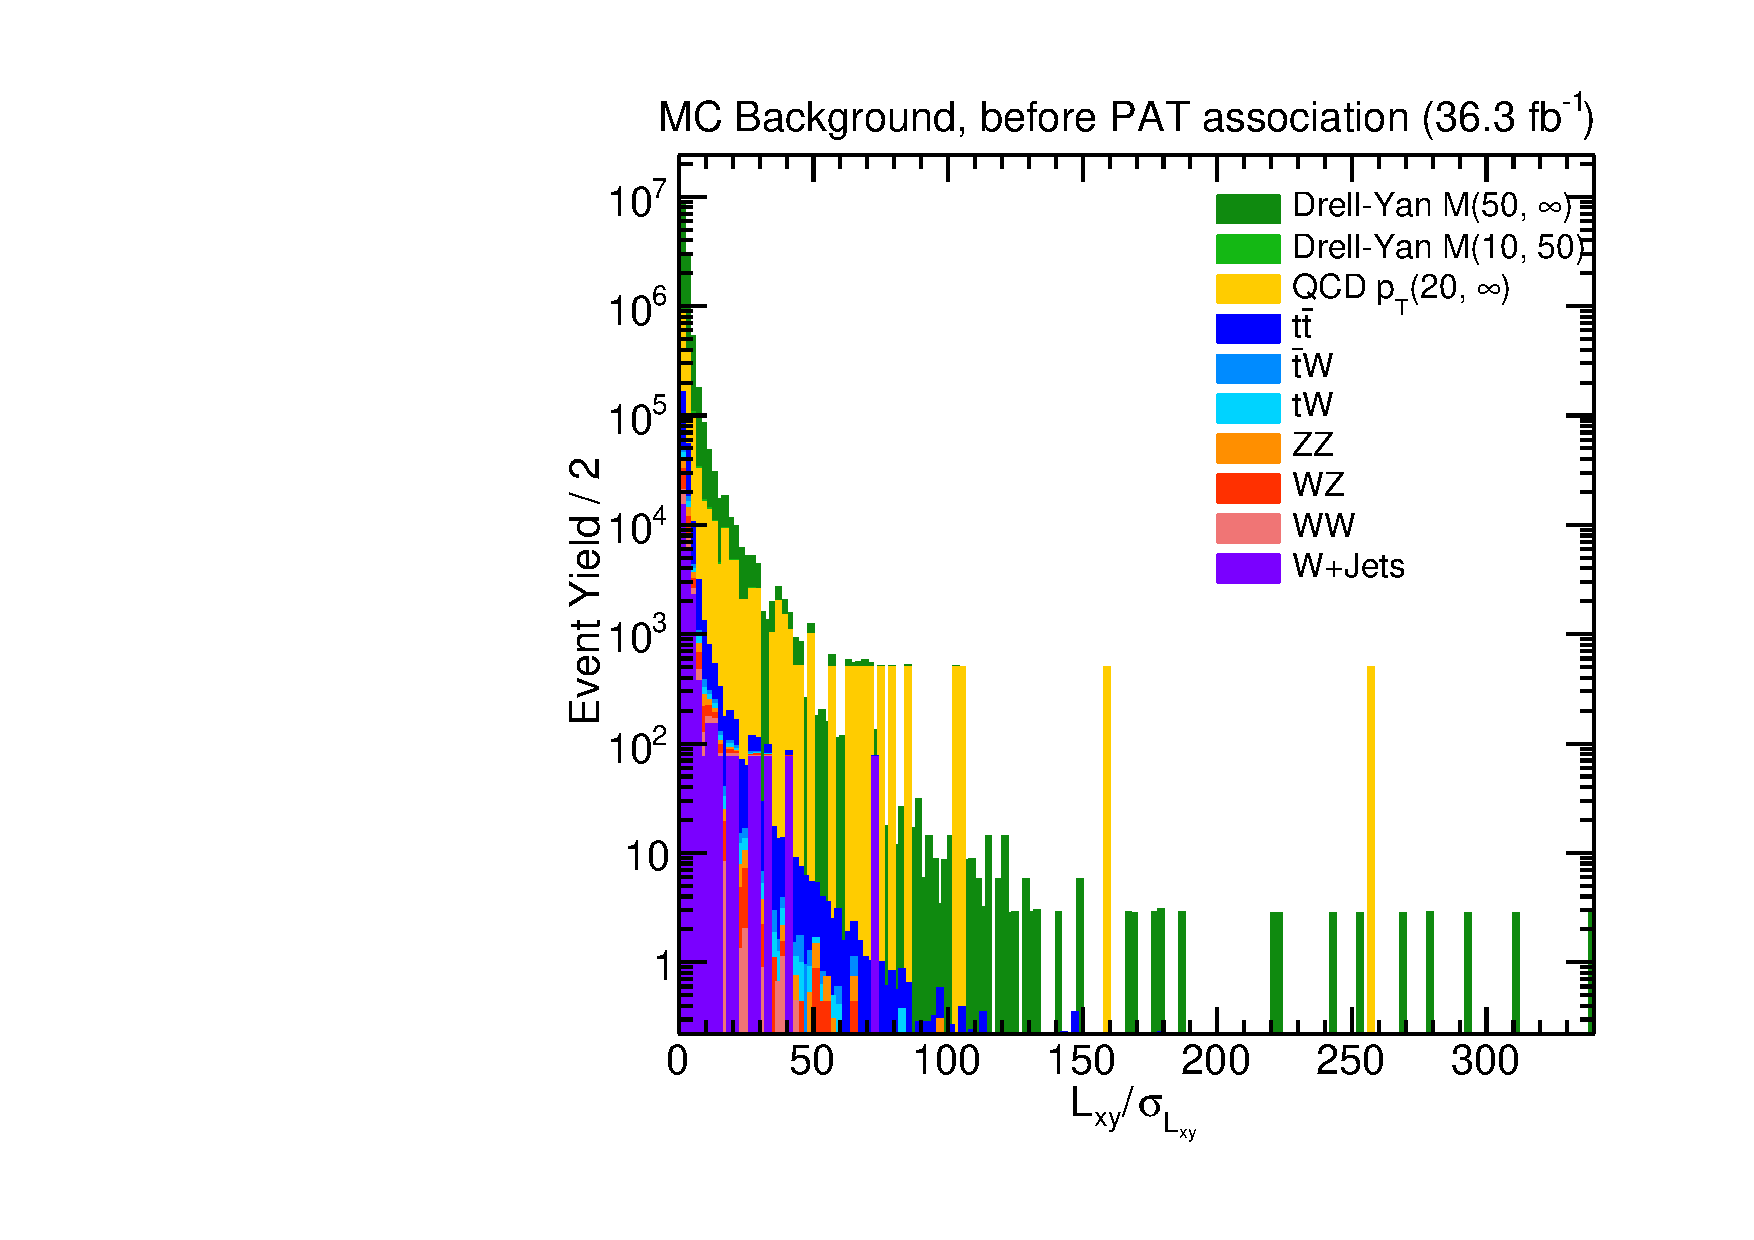
\includegraphics[width=\DSquareWidth]{figures/displaced/REPEFF_MC_LxySig-before.pdf}
  \hspace*{-2em}
  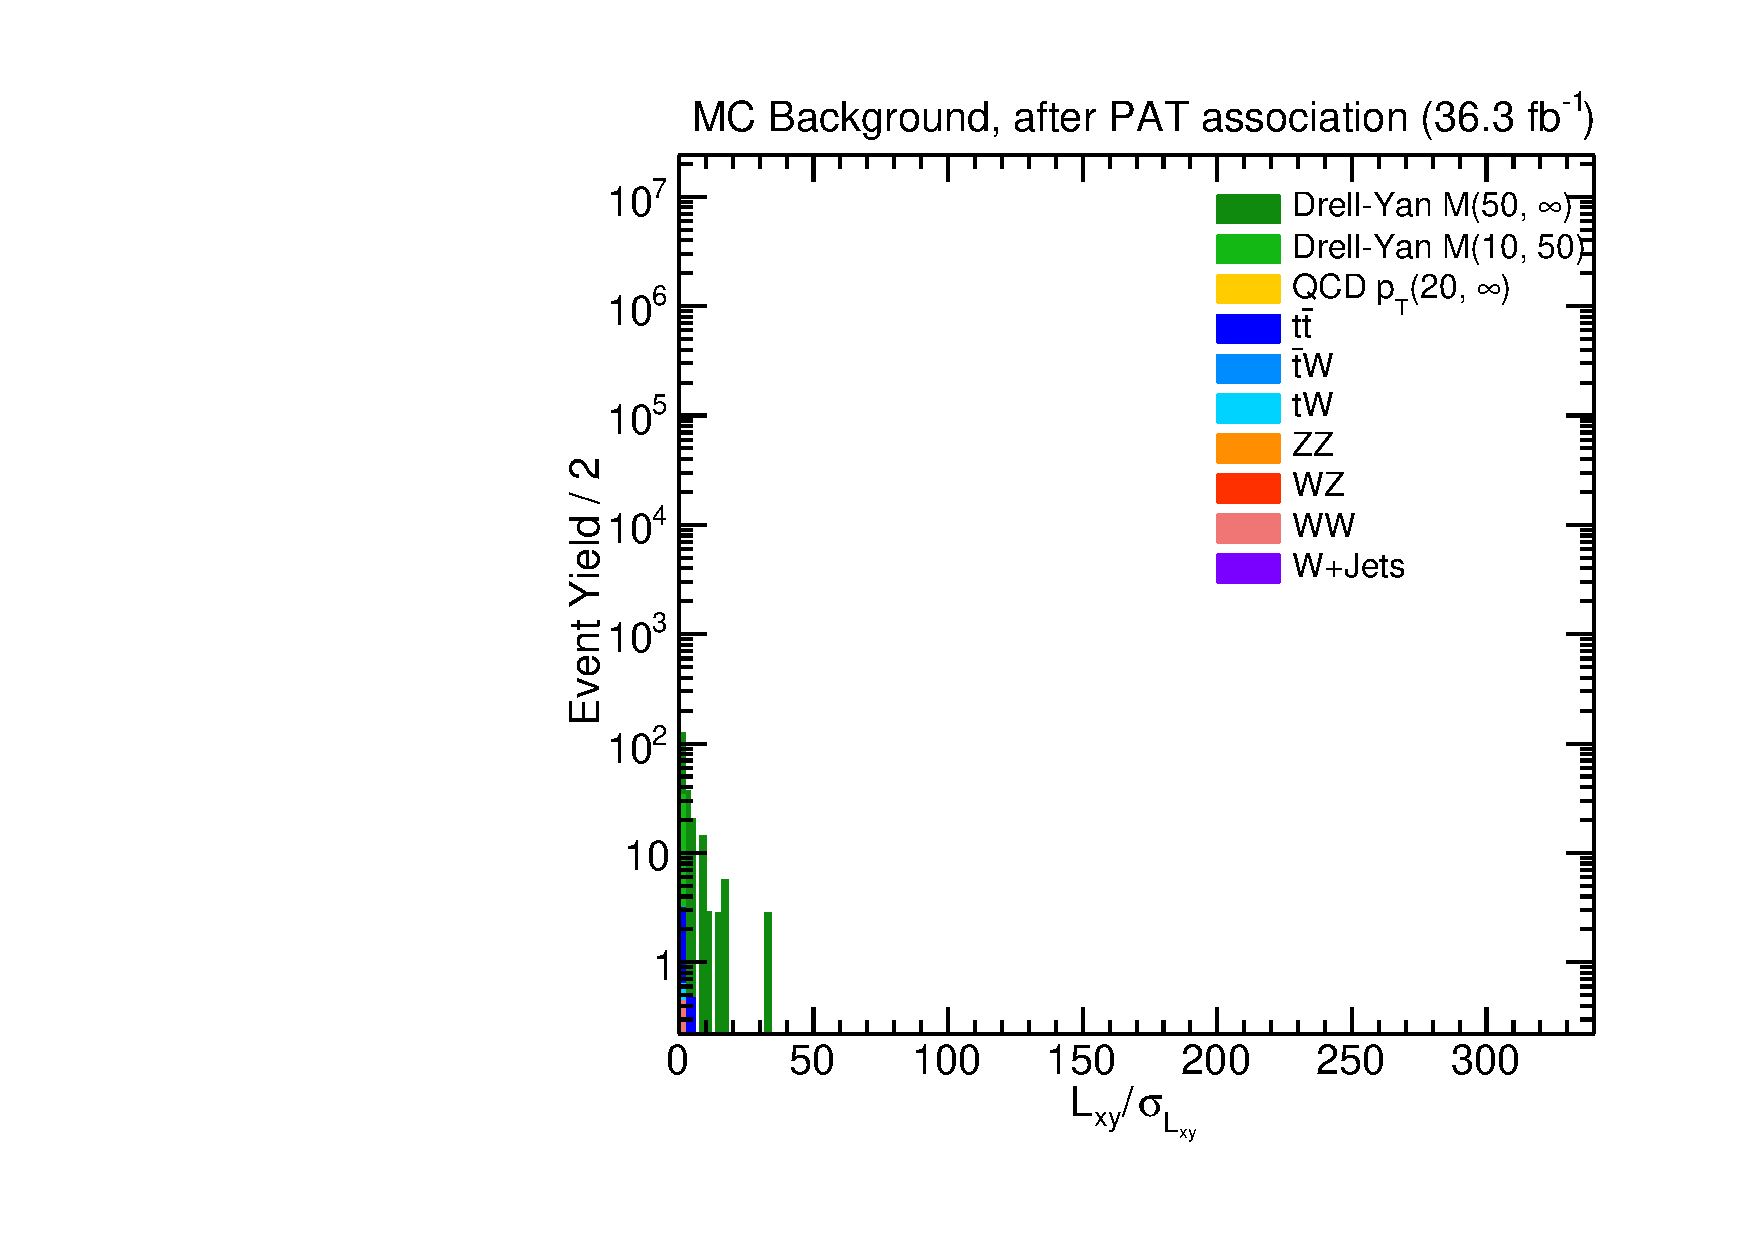
\includegraphics[width=\DSquareWidth]{figures/displaced/REPEFF_MC_LxySig-after.pdf}
  \caption{Distribution of dimuon $\Lxy/\LxyErr$ in MC background samples, scaled to 2016 integrated luminosity, (left) before and (right) after the PAT association procedure. The procedure suppresses the number of background events by a factor of $10^5$.}
  \label{fig:dd:REPEFF_MC_LxySig}
\end{figure}
\begin{figure}[p]
  \centering
  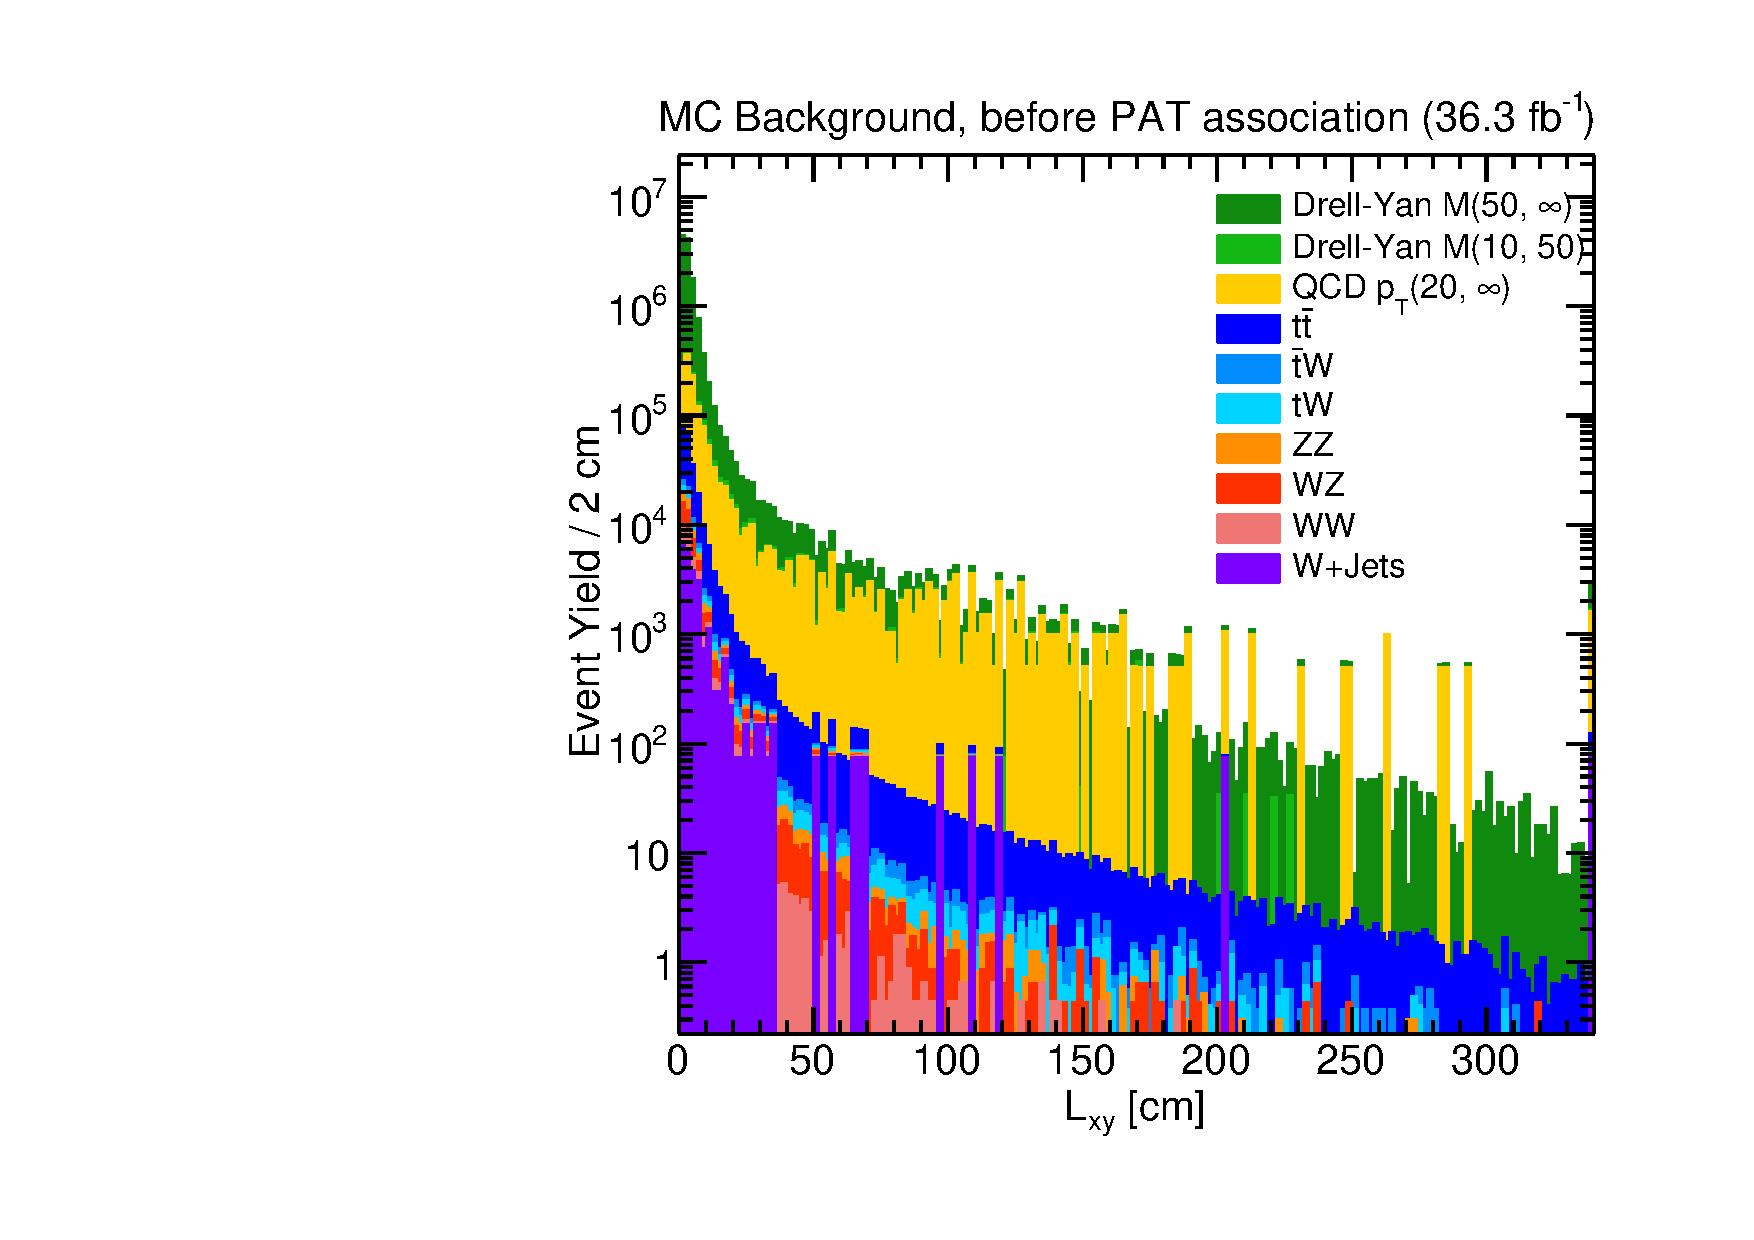
\includegraphics[width=\DSquareWidth]{figures/displaced/REPEFF_MC_Lxy-before.pdf}
  \hspace*{-2em}
  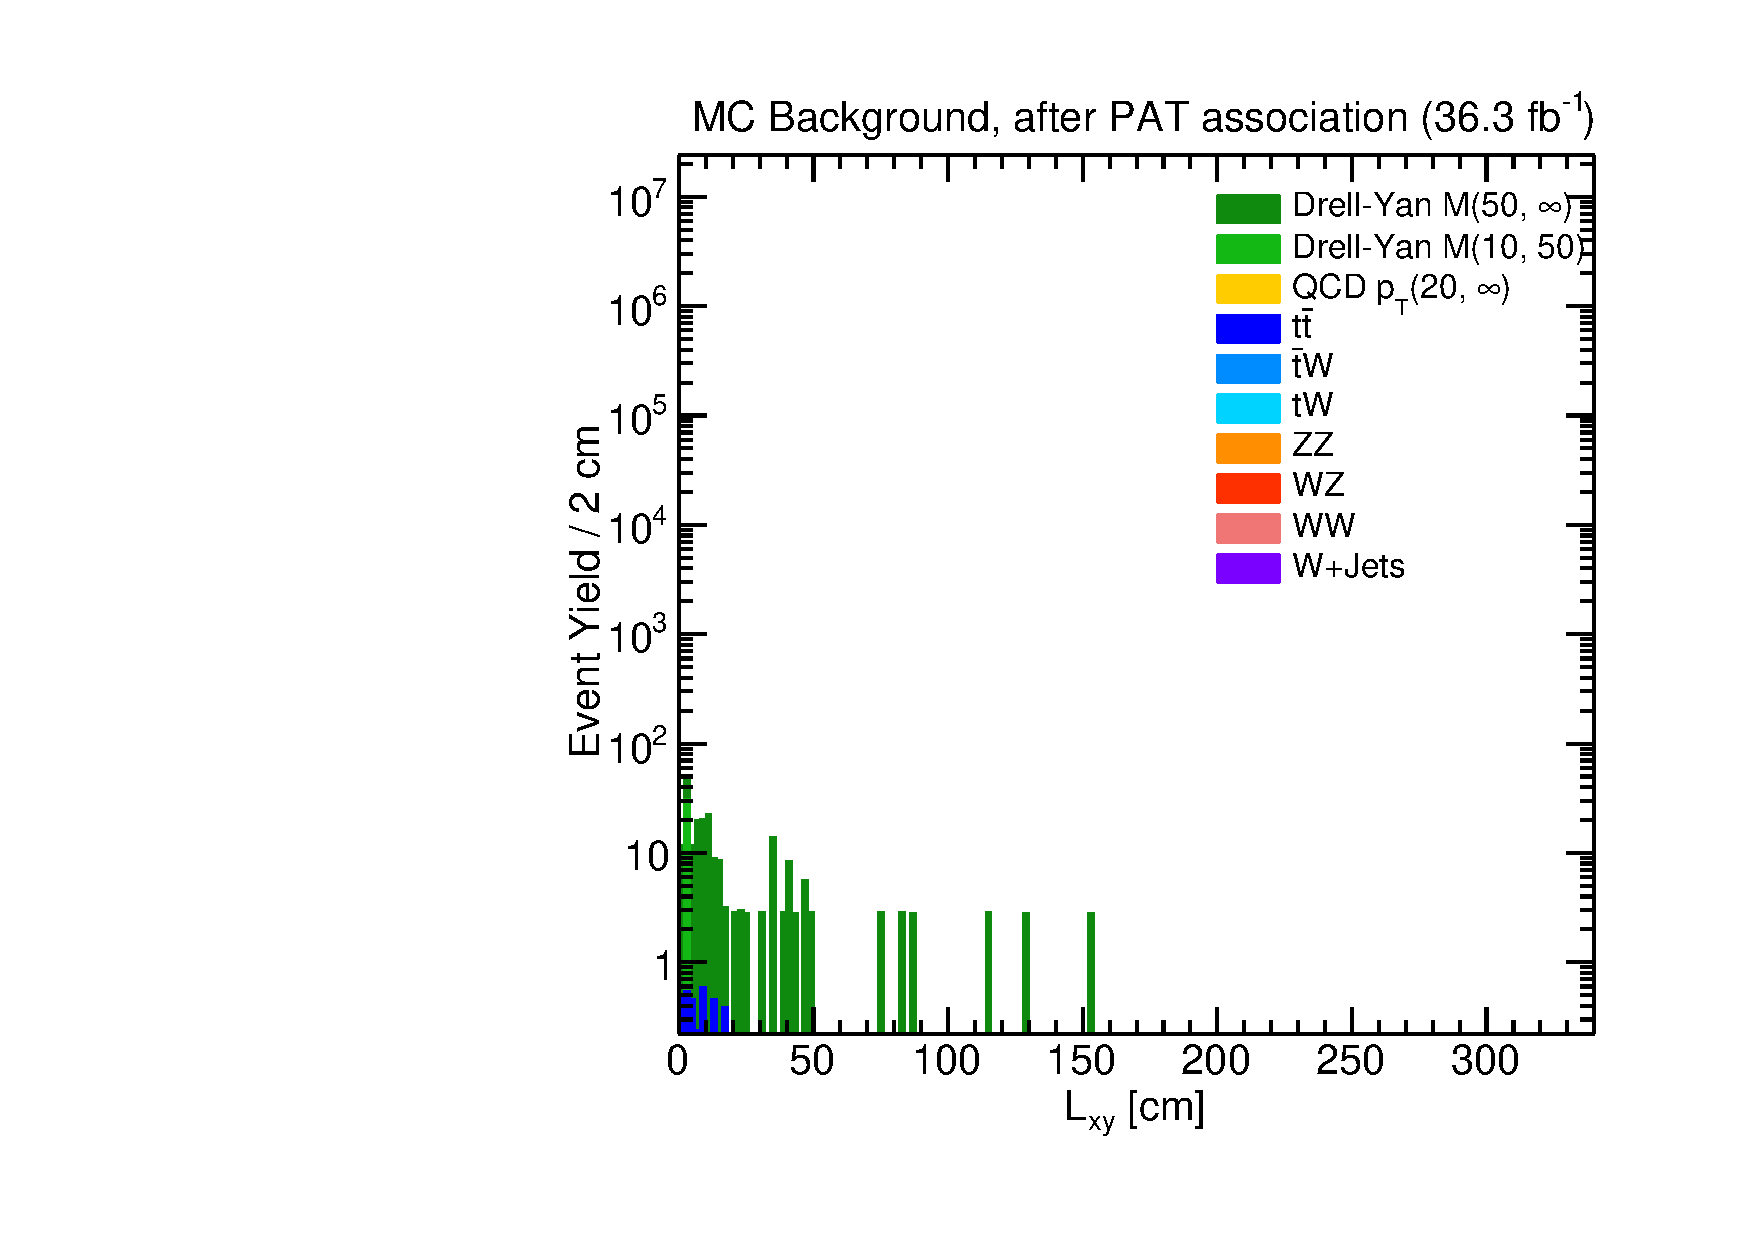
\includegraphics[width=\DSquareWidth]{figures/displaced/REPEFF_MC_Lxy-after.pdf}
  \caption{Distribution of dimuon \Lxy in MC background samples, scaled to 2016 integrated luminosity, (left) before and (right) after the PAT association procedure. The procedure suppresses the number of background events by a factor of $10^5$.}
  \label{fig:dd:REPEFF_MC_Lxy}
\end{figure}

In contrast, the association procedure essentially leaves true signal events with dimuon decays outside the tracker relatively untouched.
\Fig~\ref{fig:dd:REPEFF_Signal_Lxy} is a graph of the number of dimuons (matched to generated signal muons by choosing the closest DSA muons to each generated muon in a cone of $\deltaR < 0.2$ between their momentum directions) remaining after PAT association (\ie composed of DSA muons not associated to PAT muons), divided by the number of dimuons before PAT association, as a function of generated \Lxy.
In order to observe sufficient statistics, all 33 of the \twoMu signal samples were combined together for these graphs.
The association efficiently rejects signal events with decays inside the tracker volume, $\Lxy < 65\cm$, while rejecting no more than 5\% of signal events with decays outside the tracker volume, $\Lxy > 65\cm$.
\begin{figure}[htpb]
  \centering
  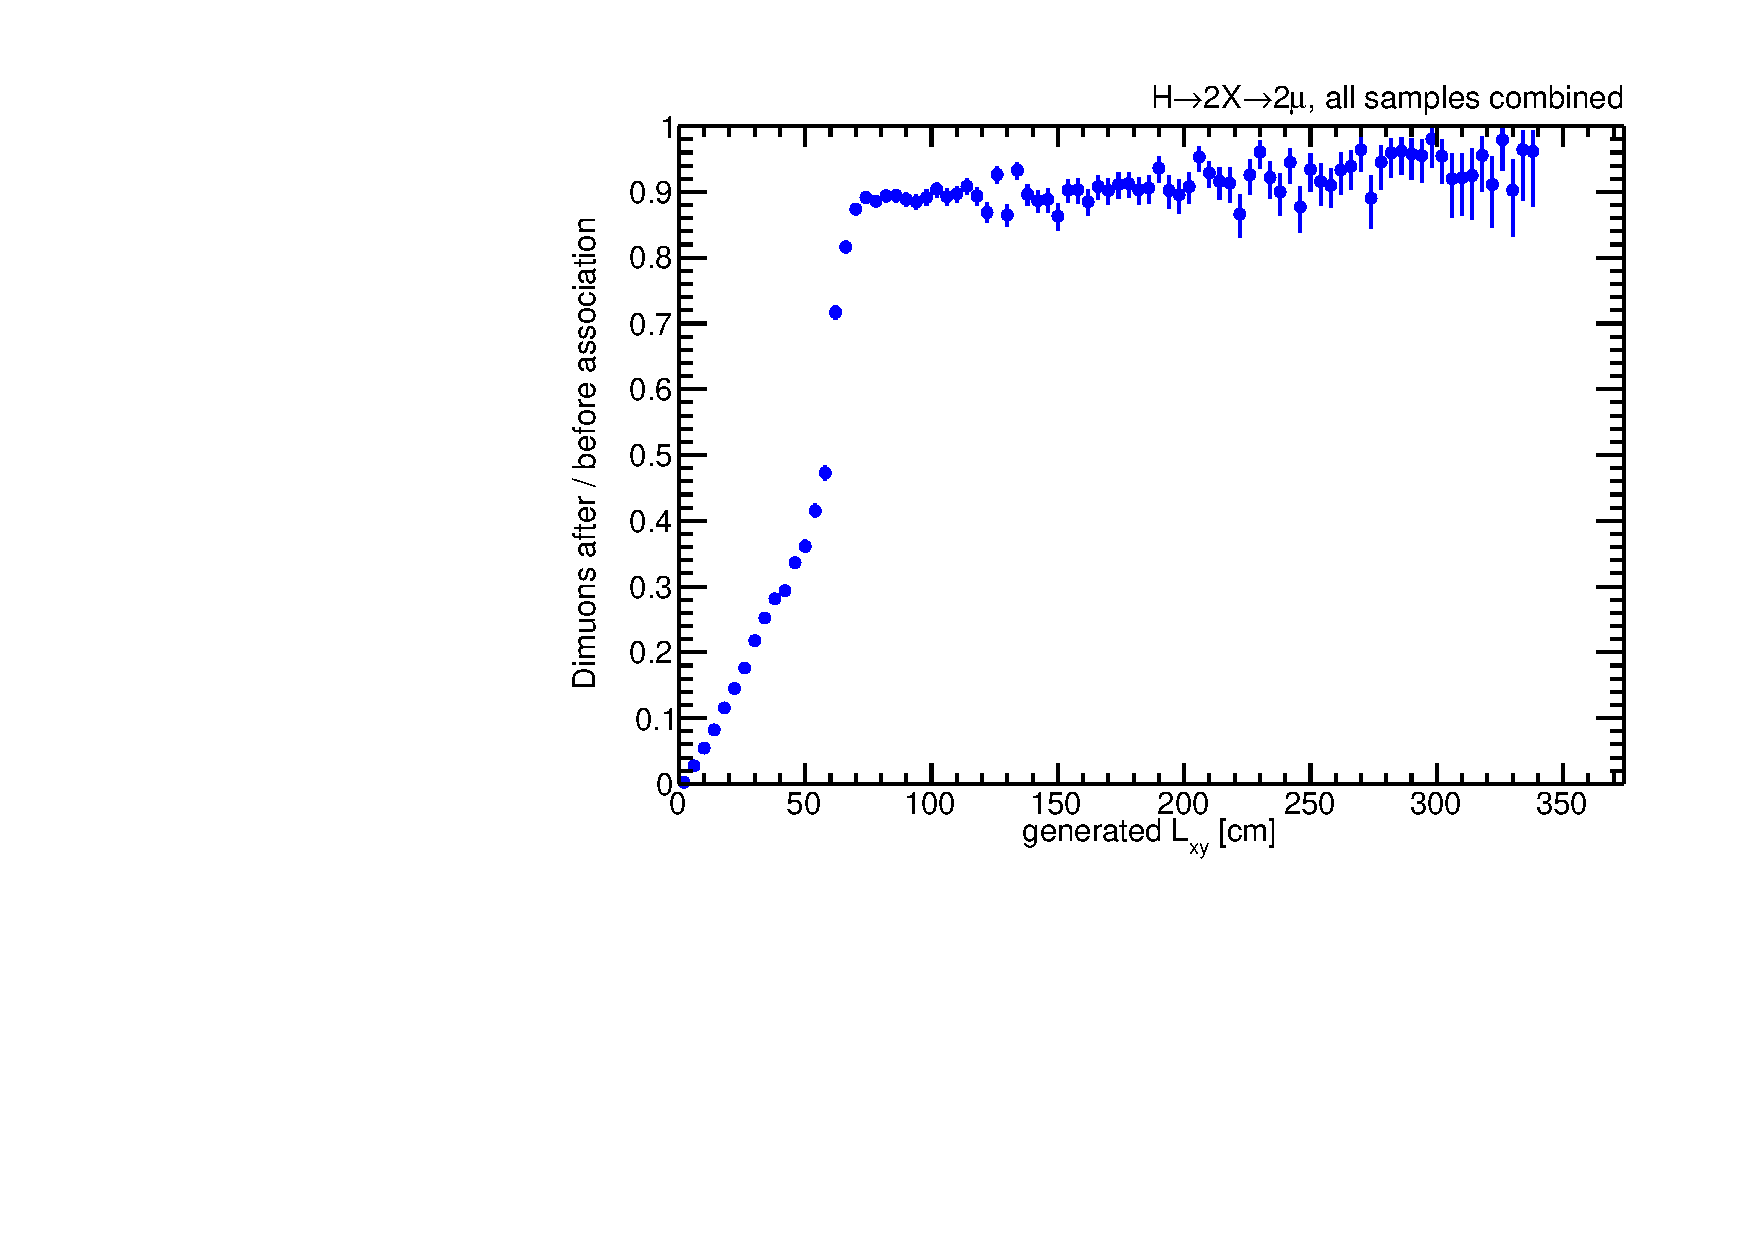
\includegraphics[width=\DFigWidth]{figures/displaced/REPEFF_Signal_Global.pdf}
  \caption{Graph of the number of dimuons after the PAT association divided by the number of dimuons before the PAT association, as a function of generated \Lxy, in all \twoMu signal samples combined. This graph shows that the association performs as expected, primarily rejecting signal events whose decays occurred within the tracker volume, while accidentally replacing no more than 5\% of events outside the tracker volume.}
  \label{fig:dd:REPEFF_Signal_Lxy}
\end{figure}


\subsection{DSA Muon Object Selection}
\label{sec:dd:DSAObject}
After the \DSAToPAT association step explained in the previous section, the analysis considers DSA muons not associated to any PAT muons.
As DSA muons are not used by many CMS analyses, a standard set of selections to identify DSA muons does not exist.
In order to further select high-quality DSA muons as well as to discriminate signal-like events from background-like events, the following requirements, along with the DSA muon preselection cuts explained in \Sec~\ref{sec:dd:DSAQuality}, serve as the DSA muon identification selection.
DSA muons are required to have
\begin{itemize}
  \item muon $\pT$ of at least 10\GeV, \ie $$\pT > 10\GeV$$
  \item \normchisq of the muon track fit of at most 4, \ie $$\chisq_\text{track}/\text{dof} < 4$$
  \item at least 19 hits in the DTs for muons reconstructed only in the barrel, \ie $$N(\text{CSC hits}) = 0 \implies N(\text{DT hits}) > 18$$
\end{itemize}

The \pT cut suppresses background events, which often have poor quality muons with low \pT, including background events arising from QCD processes.
The track \normchisq cut ensures that the muons are reasonably well reconstructed.
The $N(\text{DT hits})$ cut discriminates signal events from background events.

\subsection{Dimuon Formation from Common Vertex Fit}
\label{sec:dd:DimVertex}
A decay of a long-lived particle to two muons is detected as a pair of muons originating from a common vertex, so at this stage, pairs of reconstructed muons are investigated together for consistency with originating from a common vertex and from the decay of a massive, long-lived particle.
A pair of DSA muon tracks fit to a common vertex, along with the four-momentum sum of the two muons, is referred to as a dimuon.
All $n(n-1)/2$ possible pairs of distinct DSA muons among $n$ selected DSA muons are initially considered when forming dimuons.
This set of pairs is immediately filtered by requiring that the distance of closest approach (DCA) of the two DSA tracks helically extrapolated in the magnetic field is less than 50\unit{cm}:
$$\text{DCA} < 50\unit{cm}$$
This is a loose requirement ensuring that the common vertex fit is not performed on a pair of tracks that never come close to approaching each other.

\subsubsection{Vertex Fitting}
\label{sec:dd:VertexFitting}
The common vertex fit is performed by an implementation of the Kalman filter algorithm in the CMS software, called the \Code{KalmanVertexFitter} \cite{Fruhwirth:1987fm,Speer:927395}.
The default implementation in the CMS software version used in this analysis restricts the range of the location of the fitted vertex to approximately within the boundary of the silicon tracker.
In this analysis, this restricted range is extended to the beginning of the muon system in order to efficiently reconstruct a common vertex for particles decaying outside the tracker.

The technical changes to the CMS software are documented here.
The following changes were made to \Code{RecoVertex/VertexTools/src/SequentialVertexFitter.cc}:
\begin{itemize}
  \item \Code{TrackerBoundsRadius} was changed from 112 to 500
  \item \Code{TrackerBoundsHalfLength} was changed from 273.5 to 1000
\end{itemize}

The results of the common vertex fit are used to define the notions of dimuon quantities, such as transverse decay length.
As the existence of a common vertex fit is necessary to further study dimuon properties and consistency, the common vertex fit is required to converge.
The common vertex fit modifies the input tracks in order to be consistent with originating from a common vertex; these tracks are referred to as ``vertex-constrained'', and any of the muon properties (\pT, direction, \etc) may be different in the vertex-constrained version of the track than in the original version.
For many purposes, the vertex-constrained tracks are preferable because they represent a reconstruction performed with more information.
However, in a few situations, the vertex fitter fails or produces nonsensical results.
A few of the features of the fitter are documented here.

\begin{figure}[htpb]
  \centering
  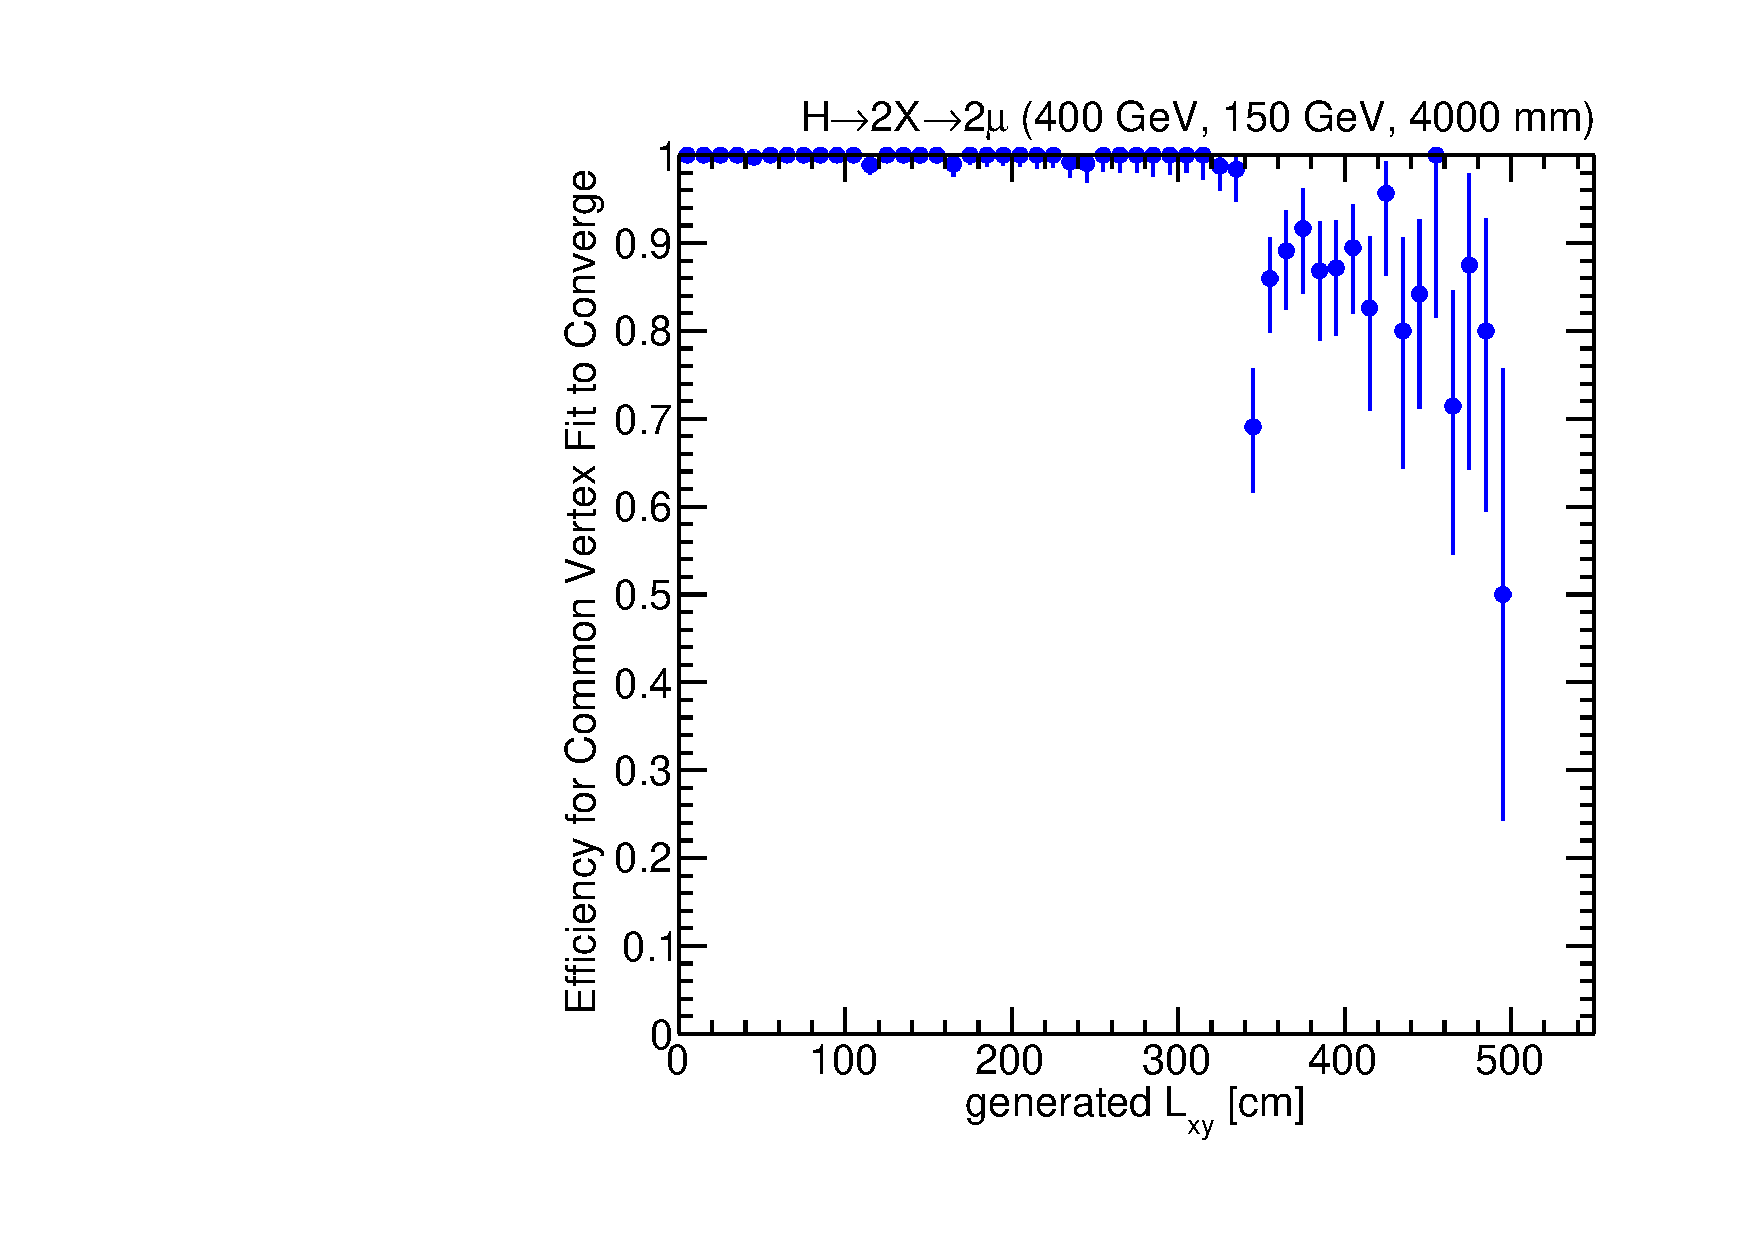
\includegraphics[width=\DSquareWidth]{figures/displaced/VFE_Lxy_2Mu2J_400_150_4000.pdf}
  \hspace*{-2em}
  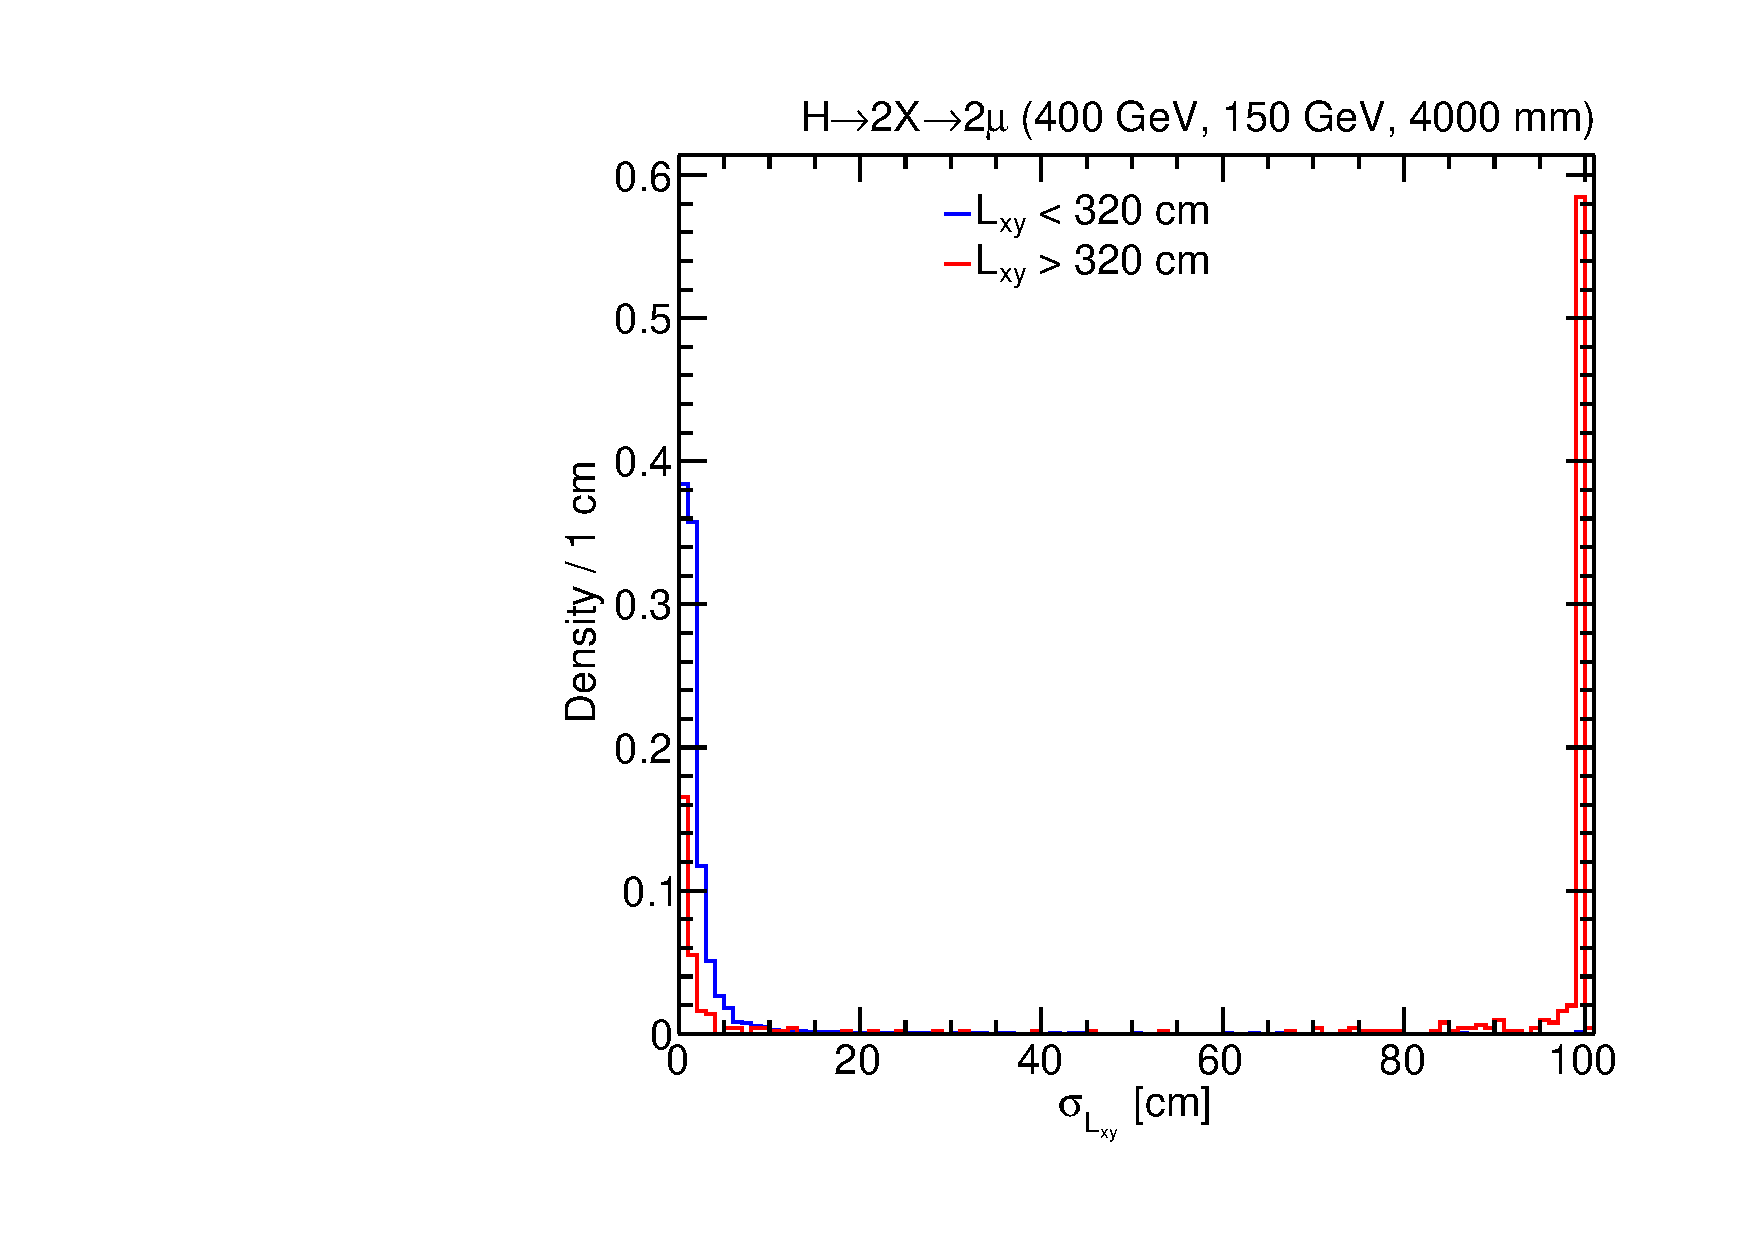
\includegraphics[width=\DSquareWidth]{figures/displaced/LESSMORE_LxyErr_2Mu2J_400_150_4000.pdf}
  \caption{(left) Efficiency for the common vertex fit to converge for the \twoMu signal sample with \FullSP{400}{150}{4000} as a function of generated \Lxy, for generated events within acceptance. Both the preselection and object selection cuts were applied to DSA muons. In this graph, events were not required to pass the trigger, the HLT-RECO matching requirement was dropped, and the \DSAToPAT association procedure was not performed. Error bars are for the statistical uncertainty only. (right) Distributions of \LxyErr normalized to unit area for the events in the numerator of the left plot, separately for $\Lxy < 320\cm$ and $\Lxy > 320\cm$, for the \twoMu signal sample with \FullSP{400}{150}{4000}, for generated events within acceptance. The distribution for $\Lxy > 320\cm$ has a large peak near 100\cm.}
  \label{fig:dd:VertexFitAnomalies}
\end{figure}

The vertex fit does not always converge for an arbitrary pair of tracks.
The left plot of \Fig~\ref{fig:dd:VertexFitAnomalies} is a graph of the efficiency for the common vertex fit to converge, with respect to signal events in which both generated muons were reconstructed as DSA muons, as a function of the generated \Lxy, for the \twoMu signal sample with \FullSP{400}{150}{4000}.

The denominator of this efficiency is the number of generated events within acceptance (both generated muon $\pT > 25\GeV$, both generated muon $|\eta| < 2$, and generated \mbox{$\Lxy < 500\cm$}) in which both generated muons had matching DSA muons.
That is, each generated muon had a DSA muon passing the muon preselection and the muon object selection within a cone of $\deltaR < 0.2$ between their momentum directions.
The numerator of this efficiency is the number of such events in which the dimuon common vertex fit converged for the two matched muons.
In order to observe the effect of the common vertex fit independently of the low trigger efficiency at large \Lxy, events were not required to pass the trigger and the HLT-RECO matching requirement was dropped.
In order to obtain sufficient statistics, the \DSAToPAT association procedure was not performed.

Convergence of the vertex fit is highly efficient when fitting two DSA muon tracks that are matched to generated signal muons produced from long-lived particle decaying in the detector up to transverse displacements of 330\unit{cm}.
Beyond 330\unit{cm}, the efficiency for the common vertex fit to converge drops dramatically.

For those events beyond 330\unit{cm} that do converge, the fit quality is often quite poor, \eg the \pT resolutions of the vertex-constrained tracks are worse than before the fit.
Finally, many of these events retain an internal \Lxy uncertainty (\LxyErr) of a default value of 100\cm.
The right plot of \Fig~\ref{fig:dd:VertexFitAnomalies} shows distributions, normalized to unit area, of the events in the numerator of the left plot of \Fig~\ref{fig:dd:VertexFitAnomalies}, separately for $\Lxy < 320\cm$ and $\Lxy > 320\cm$.
A large fraction of the events with $\Lxy > 320\cm$ have \LxyErr near 100\cm.
Such events would have a small \Lxy significance (3 or less) and would not pass an analysis selection.
This type of common vertex fit failure would result in the loss of these events, even though the fit converged.

As in the Run~1 analyses, the trigger efficiency at such large \Lxy values is quite small.
Therefore, further study of these events and attempts to rescue them from the behavior of the vertex fitter are of low priority for this analysis, and the underlying causes for this behavior remain a curiosity.

\subsection{Pairing Criteria}
\label{sec:dd:PC}
Considering all possible pairs of DSA muons results in many dimuons formed from DSA muons that are not related in any way.
It is therefore important to develop criteria that choose the correct reconstructed dimuons with high efficiency, consistent with signal.
Selections on individual dimuons (such as requiring the \vchisq to be small) impose some quality constraints that are useful for selecting such dimuons, but any set of criteria that determines which pairs of muons form the correct dimuons must consider the event as a whole.
Choosing such a set of pairing criteria is particularly subtle in, for example, decays of two long-lived particles into a final state with 4 muons.
The 4 muons can be nominally paired into 6 overlapping dimuons, which can be partitioned into three distinct sets of 2 dimuons with no shared muons; the criteria must choose between them.
This situation is made more complex when, among other things,
\begin{itemize}
  \item one or more muons are not reconstructed
  \item duplicate muons are reconstructed from partial sets of hits
  \item muons are not all reconstructed with the correct charge
  \item pairs of muons are highly collimated and distinguishing them is difficult
  \item vertex fits of muons from different long-lived particle decays yield a good \vchisq
\end{itemize}
In developing this set of pairing criteria, several combinations of metrics were considered.
\begin{itemize}
  \item Dimuon(s) formed from the highest \pT muons in the event
  \item Dimuon(s) with the least \vchisq in the event
  \item Dimuon(s) formed from muons with charges of opposite sign
  \item Pairs of dimuons with the least sum of \vchisq
  \item Pairs of dimuons with the least difference in reconstructed dimuon mass
\end{itemize}
\Fig~\ref{fig:dd:pc} is a diagram illustrating the application of the pairing criteria to the set of all possible dimuons in the case of four selected muons.
\begin{figure}[htpb]
  \centering
  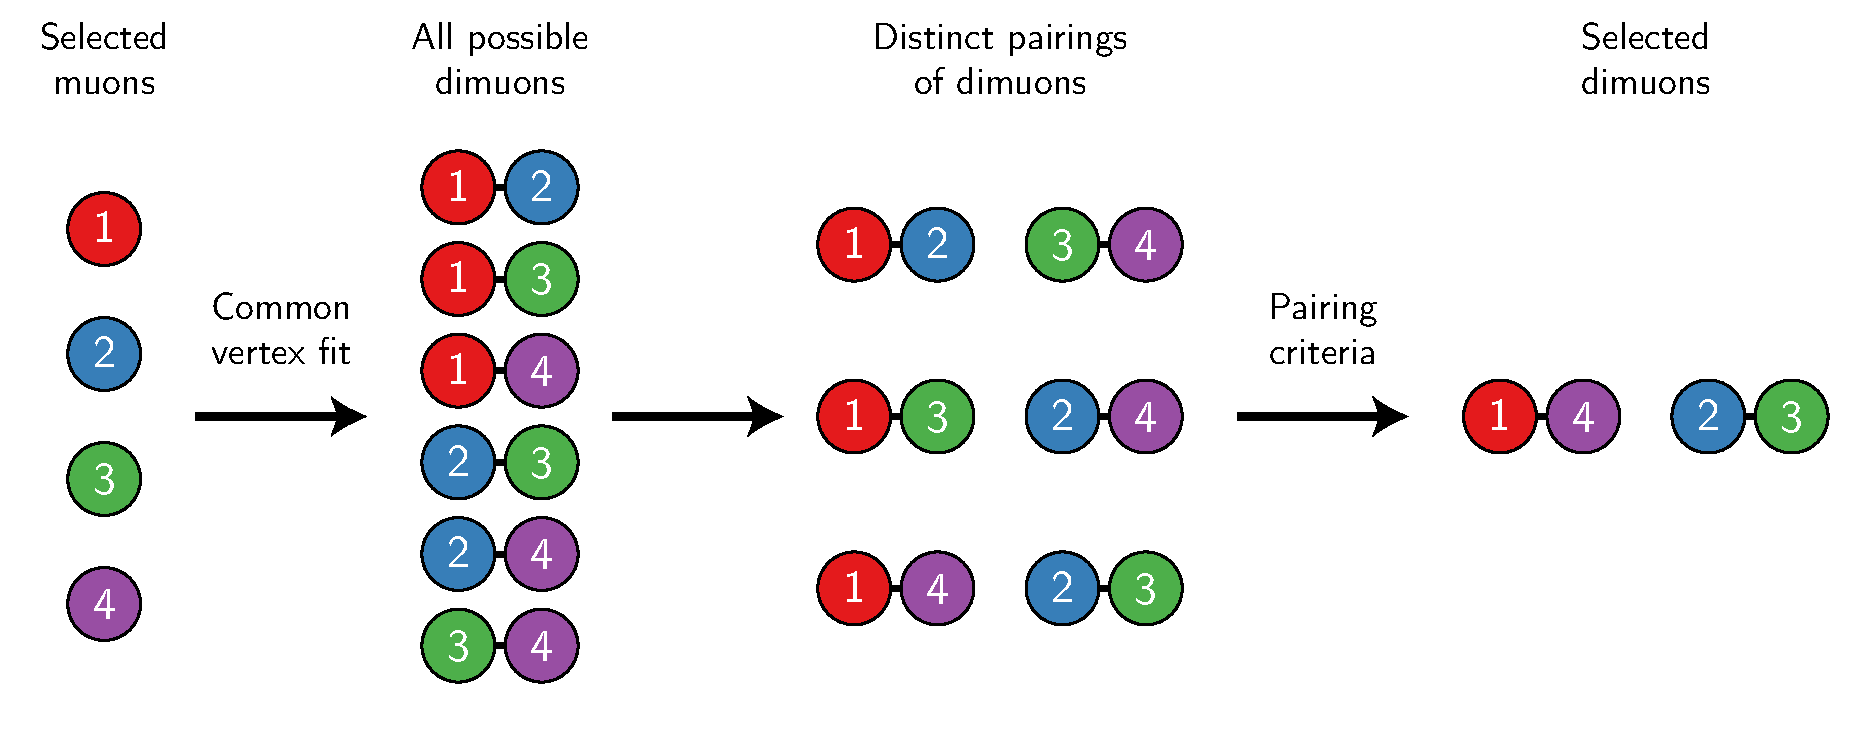
\includegraphics[width=\textwidth]{figures/displaced/PairingCriteriaDiagram.pdf}
  \caption{Diagram illustrating the application of pairing criteria to dimuons in the case of four selected muons. Four muons may be paired into six dimuons whose constituent muons overlap. These six dimuons may be partitioned into three distinct pairings of dimuons, in which no muons are shared between dimuons. Pairing criteria select the correct pair of dimuons consistent with a four muon signal event.}
  \label{fig:dd:pc}
\end{figure}

Potential pairing criteria were studied and optimized on both the \twoMu and \fourMu signal samples.
Choosing the highest \pT muons in the event is highly correlated with choosing the signal muons, a fact that is robust across all signal sample parameters covering a wide range of long-lived particle lifetimes and muon \pT spectra.
Requiring that dimuons be formed from muons of opposite charge provides only modest efficiency gains with respect to choosing the signal dimuons, and is undesirable at this stage as it introduces dependence on a specific type of signal model.
In events with fewer than four muons, a simple ranking of all possible dimuons by \vchisq yielded the highest efficiency.
The combinatorial space is far richer in events with four or more muons.
For long-lived particles decaying outside the tracker leading to events with at least 4 muons, the criterion yielding the highest efficiency to select signal dimuons is to choose the pair of dimuons whose \vchisq sum is the smallest, among all distinct pairs of dimuons that can be formed from the 4 highest \pT muons in the event. 
An alternative criterion to the least sum of \vchisq is the least difference in reconstructed dimuon mass.
Due to the limited mass resolution of DSA muons, this criterion was found to be less efficient overall than the least sum of \vchisq, except in events with a generated transverse decay length of less than 30\unit{cm}, a region where this DSA muon-based analysis has zero sensitivity.
Applying the pairing critera to an event with any number of dimuons formed from any number of muons results in 2 or fewer selected dimuons for the event.
The full technical details of this procedure are depicted in \Fig~\ref{fig:dd:pca}.

\begin{figure}[htpb]
  \centering
  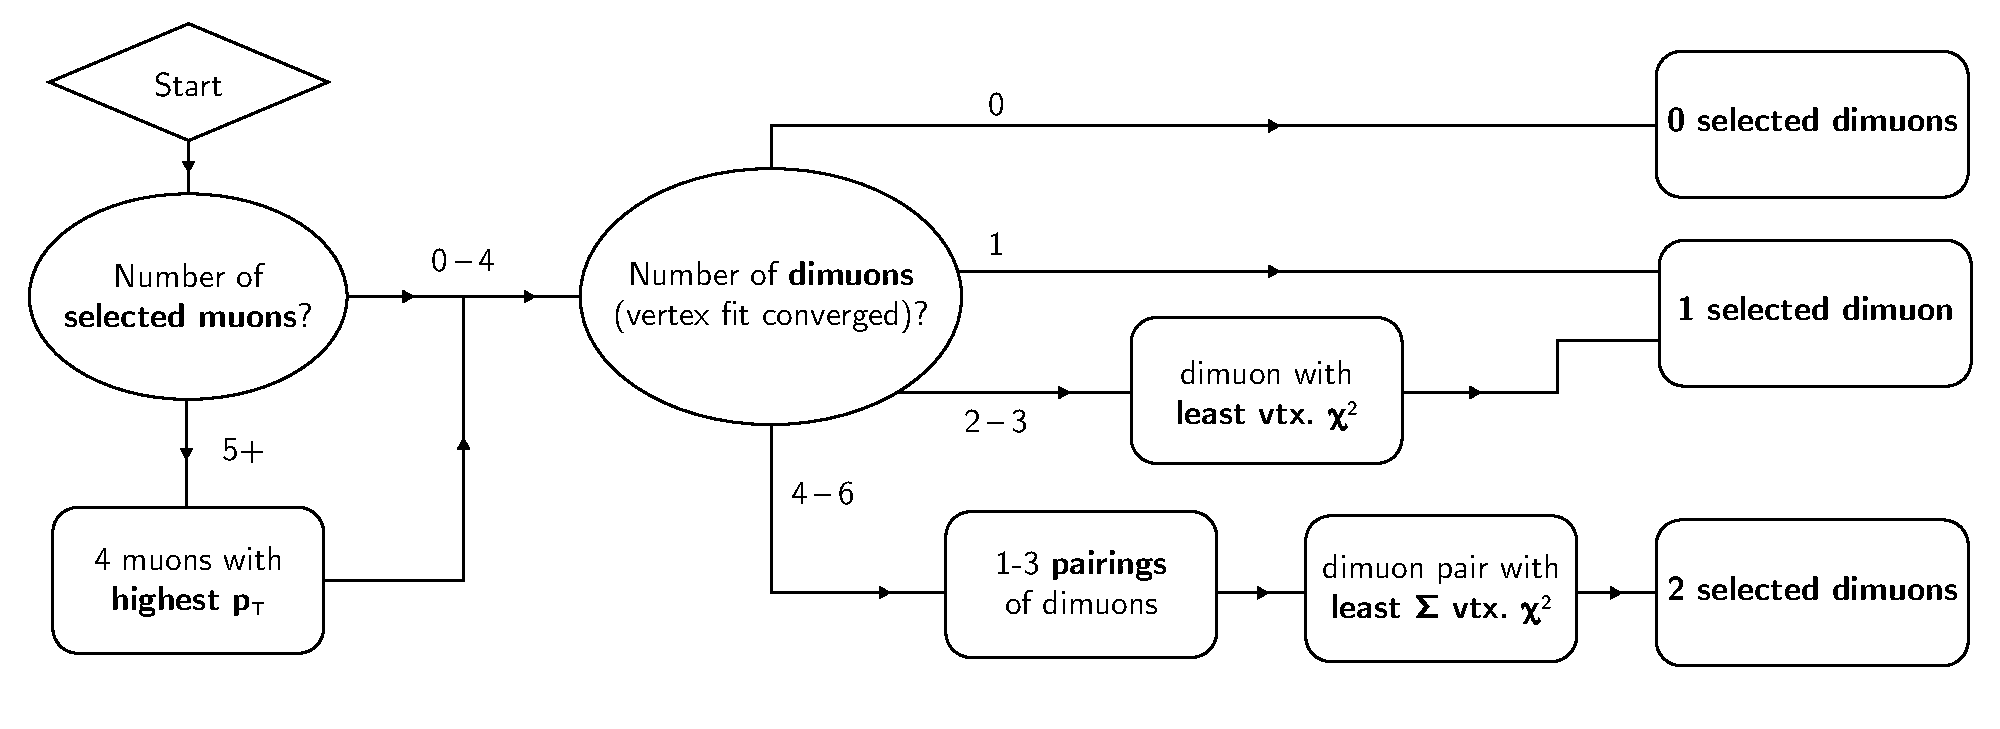
\includegraphics[width=\textwidth]{figures/displaced/PairingCriteriaAlgorithm.pdf}
  \caption{Flowchart depicting the technical details of the pairing criteria procedure. Up to 4 DSA muons are selected, ranked by \pT. With the DCA and vertex fit convergence requirements, these muons can be formed into up to 6 dimuons (0 for 0 or 1 muon, up to 1 for 2 muons, up to 3 for 3 muons, and up to 6 for 4 muons). The pairing criteria choose up to 2 dimuons among the possible dimuons.}
  \label{fig:dd:pca}
\end{figure}

\Fig~\ref{fig:dd:PC_Eff} shows graphs of the efficiency for the pairing criteria to correctly select reconstructed dimuons as a function of generated \Lxy, for a selection of \twoMu and \fourMu signal samples.
\Fig~\ref{fig:dd:PC_Eff_Global} shows the same graphs, but for all 33 signal samples combined together.
The denominator of this efficiency is the number of generated signal dimuons matching a reconstructed dimuon (using the closest DSA muons to each generated muon in a cone of $\deltaR < 0.2$ between their momentum directions).
The numerator of this efficiency is the number of reconstructed dimuons chosen by the pairing criteria that were the same as the reconstructed dimuon matched to generated signal.
This efficiency is 97--100\% for \twoMu and 80--98\% for \fourMu signal samples with medium and long lifetimes, for generated transverse decay lengths of $\Lxy > 100 \cm$.
The pairing criteria are less efficient for \fourMu samples with larger values of \mH and smaller values of \mX, because events in such samples consist of two pairs of highly collimated muons, which yield a greater uncertainty in the fitted vertex position in the dimuon momentum direction, and therefore less discriminating vertex \chisq values.

\begin{figure}[p]
  \centering
  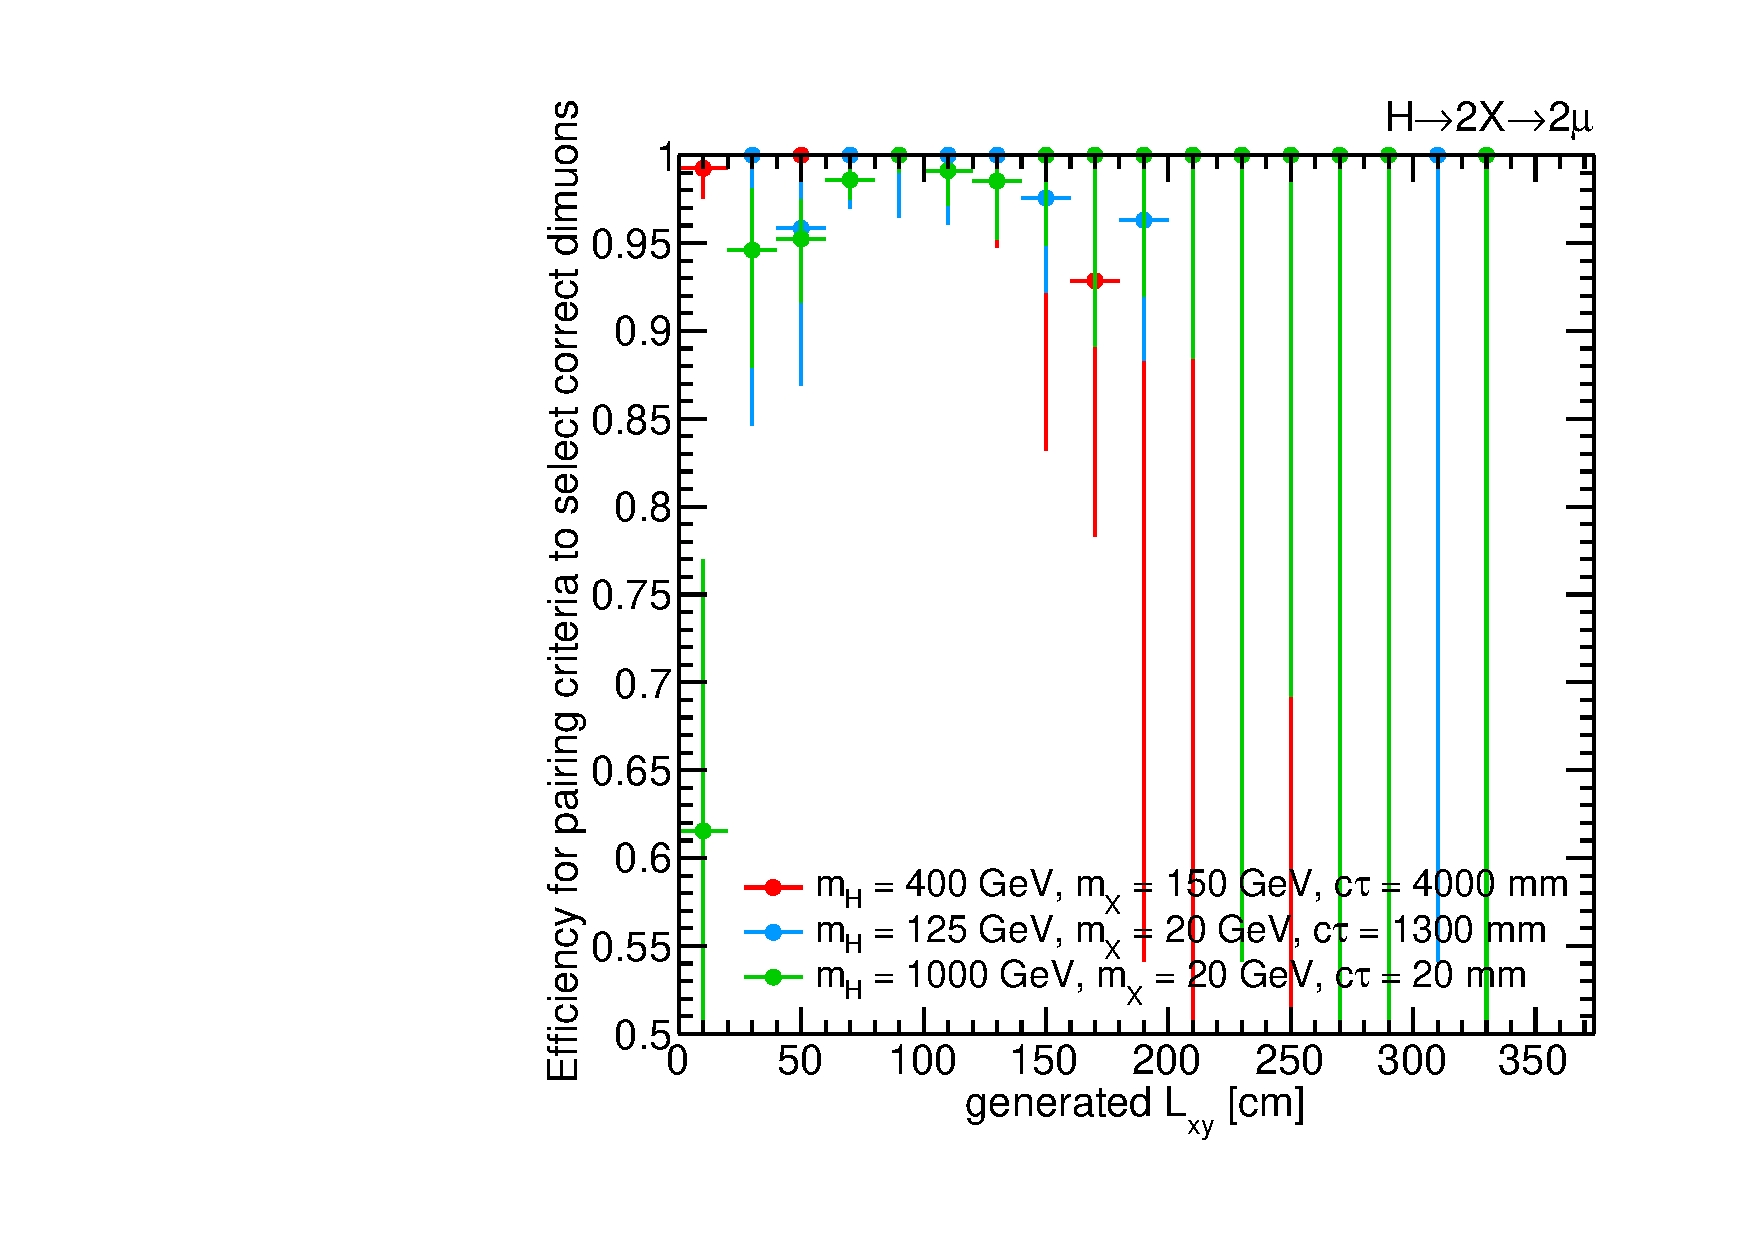
\includegraphics[width=\DSquareWidth]{figures/displaced/PC_Lxy_2Mu2J_Mul.pdf}
  \hspace*{-2em}
  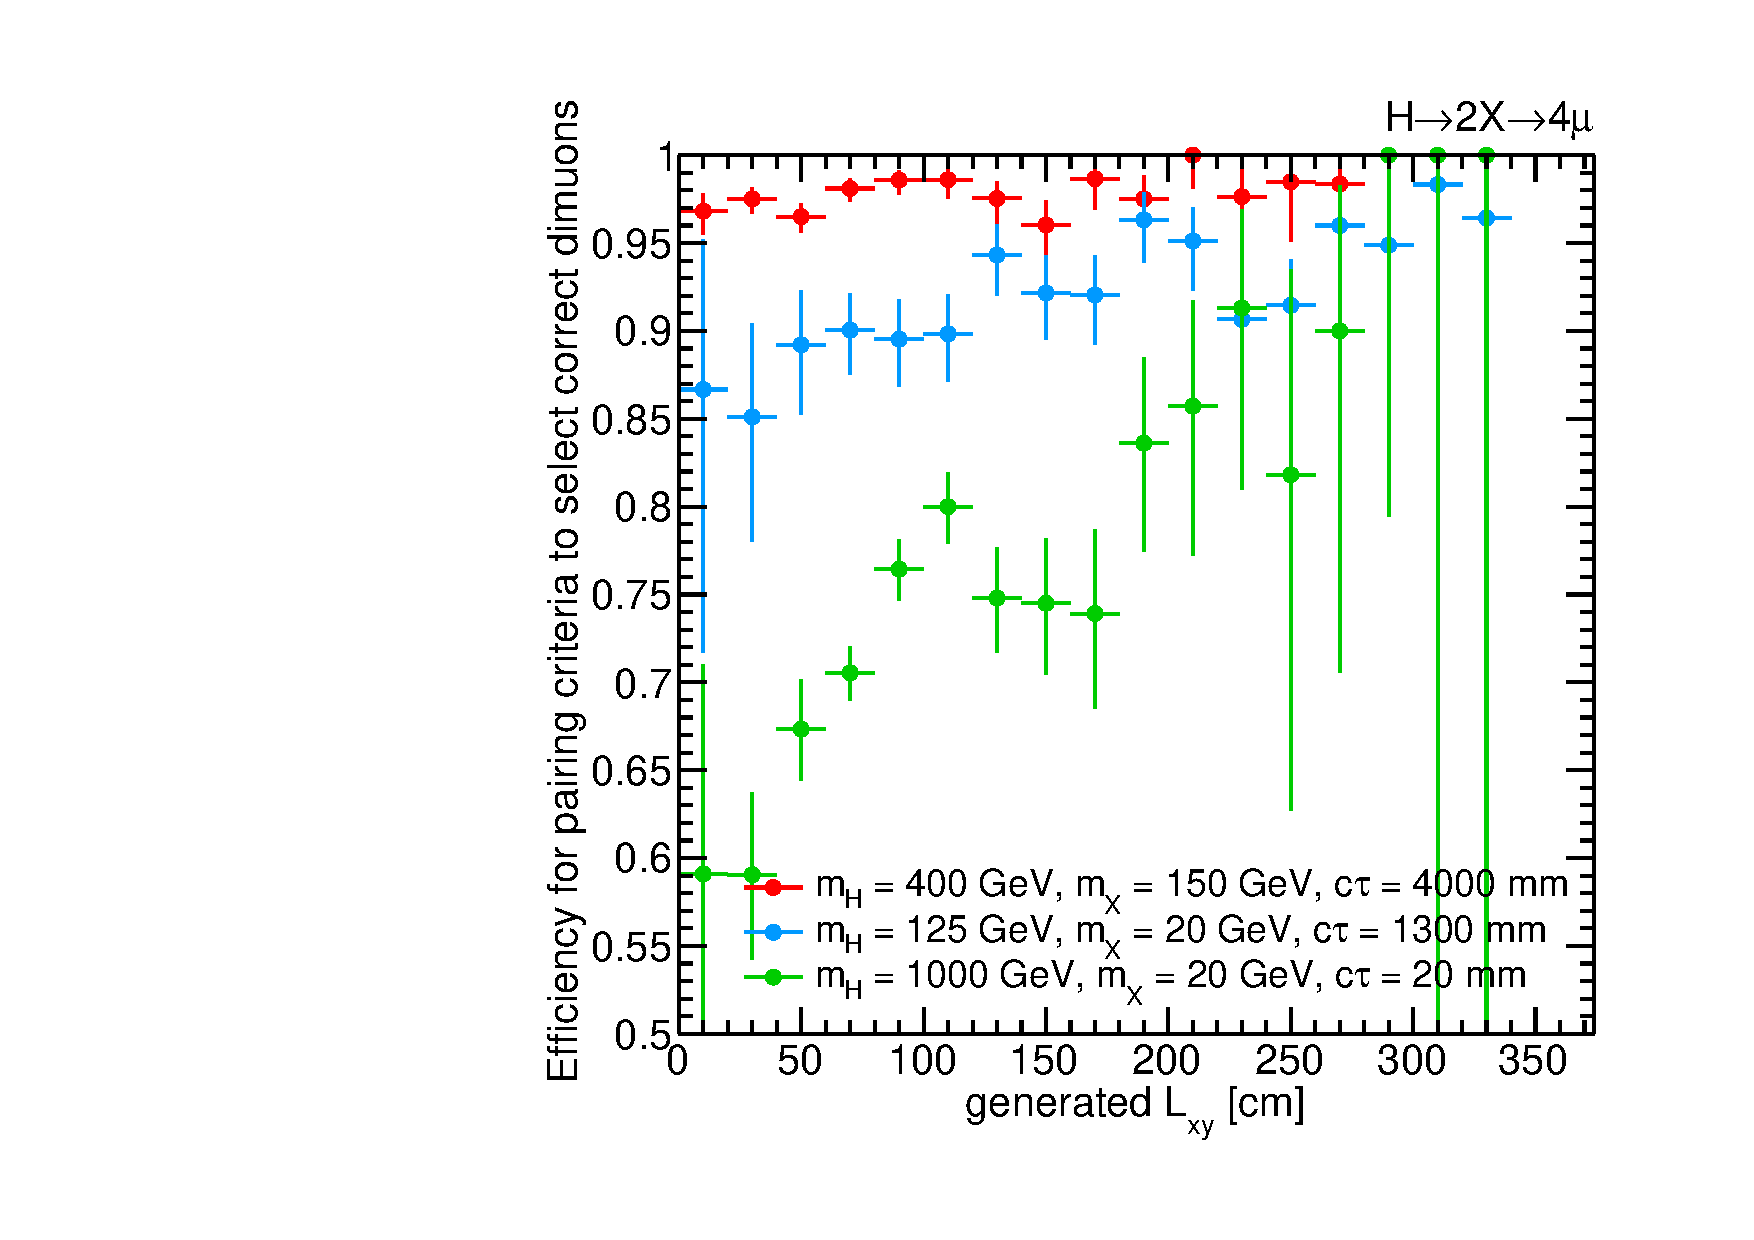
\includegraphics[width=\DSquareWidth]{figures/displaced/PC_Lxy_4Mu_Mul.pdf}
  \caption{Efficiency for the pairing criteria to correctly choose reconstructed dimuons as a function of generated \Lxy for (left) \twoMu signal samples and (right) \fourMu signal samples, for selected signal parameters. The behavior varies with signal parameters, and is lower for \fourMu signal samples, but overall the efficiency is high outside the tracker volume ($\Lxy > 100\cm$).}
  \label{fig:dd:PC_Eff}
\end{figure}
\begin{figure}[p]
  \centering
  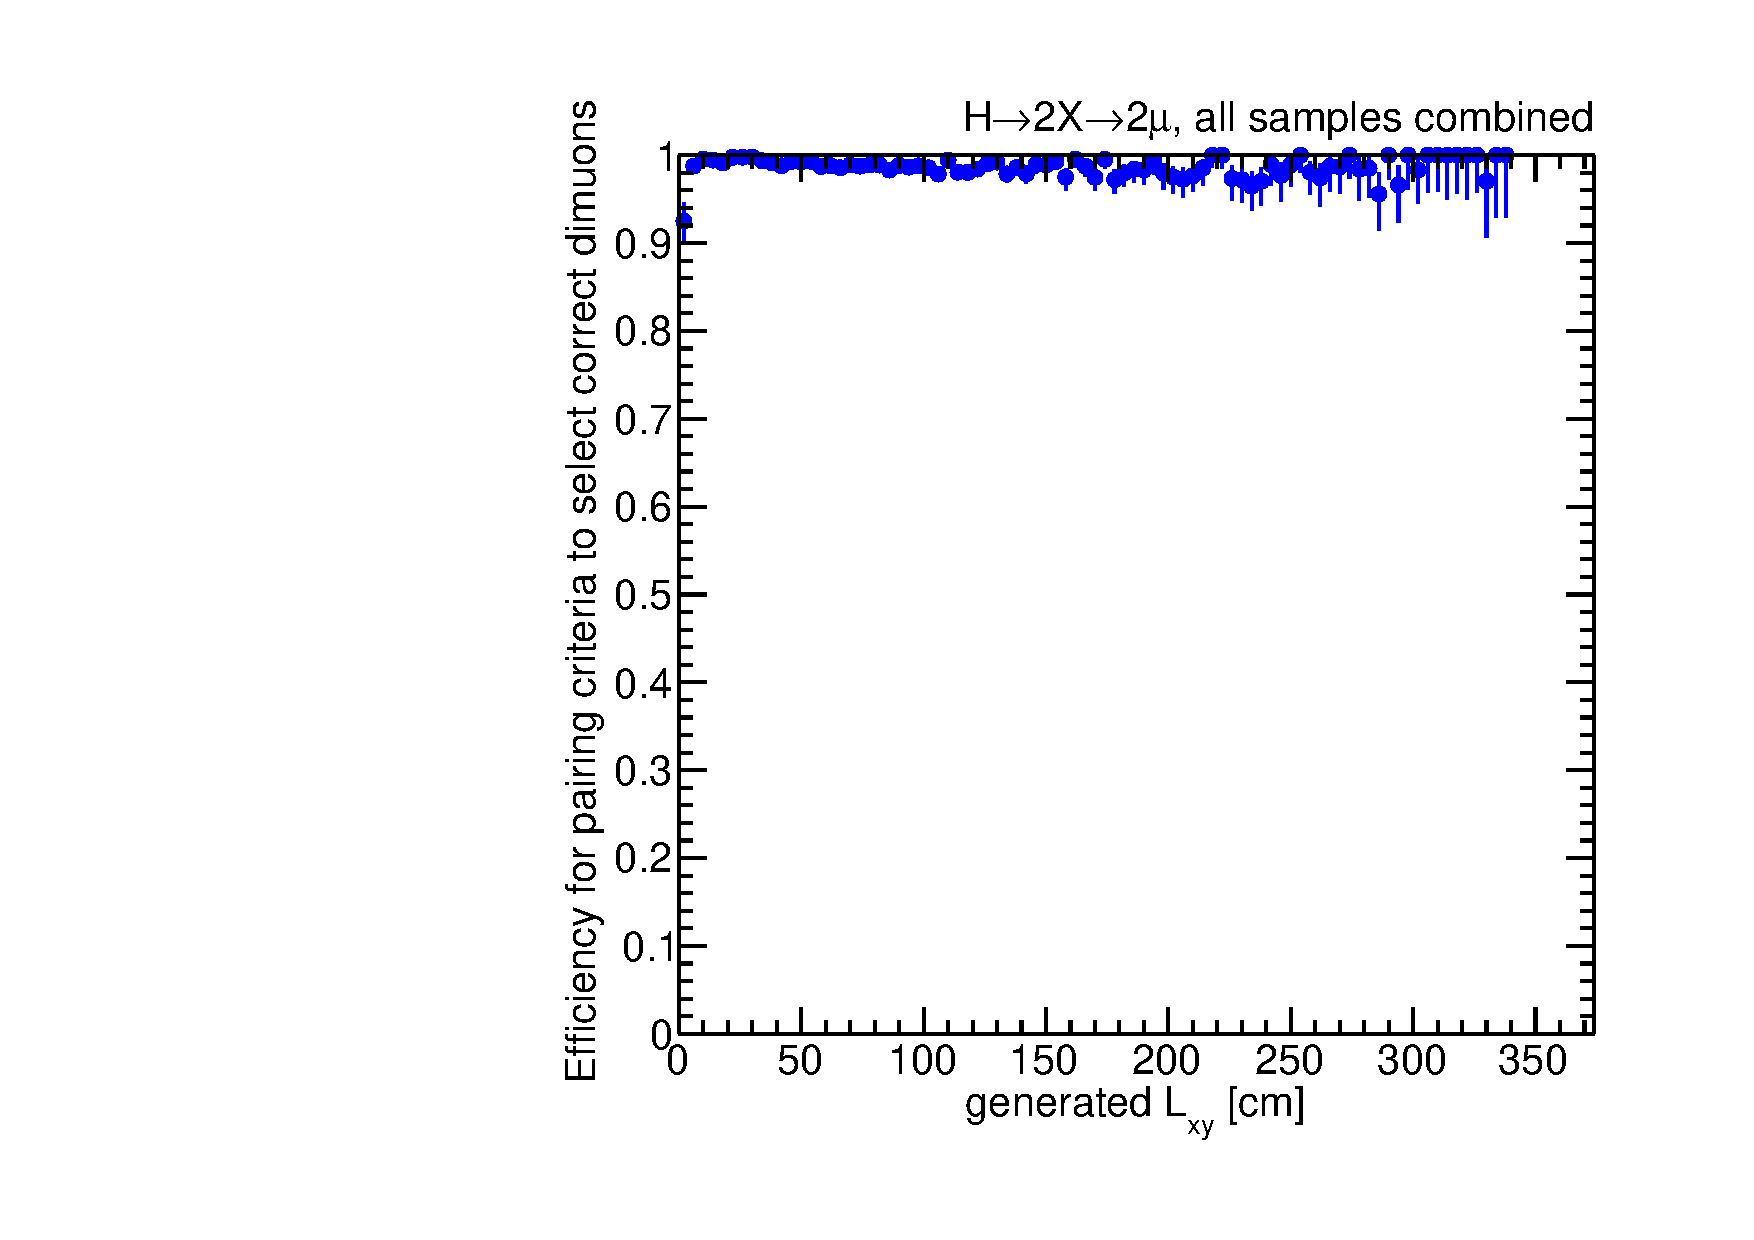
\includegraphics[width=\DSquareWidth]{figures/displaced/PC_Lxy_2Mu2J_Global.pdf}
  \hspace*{-2em}
  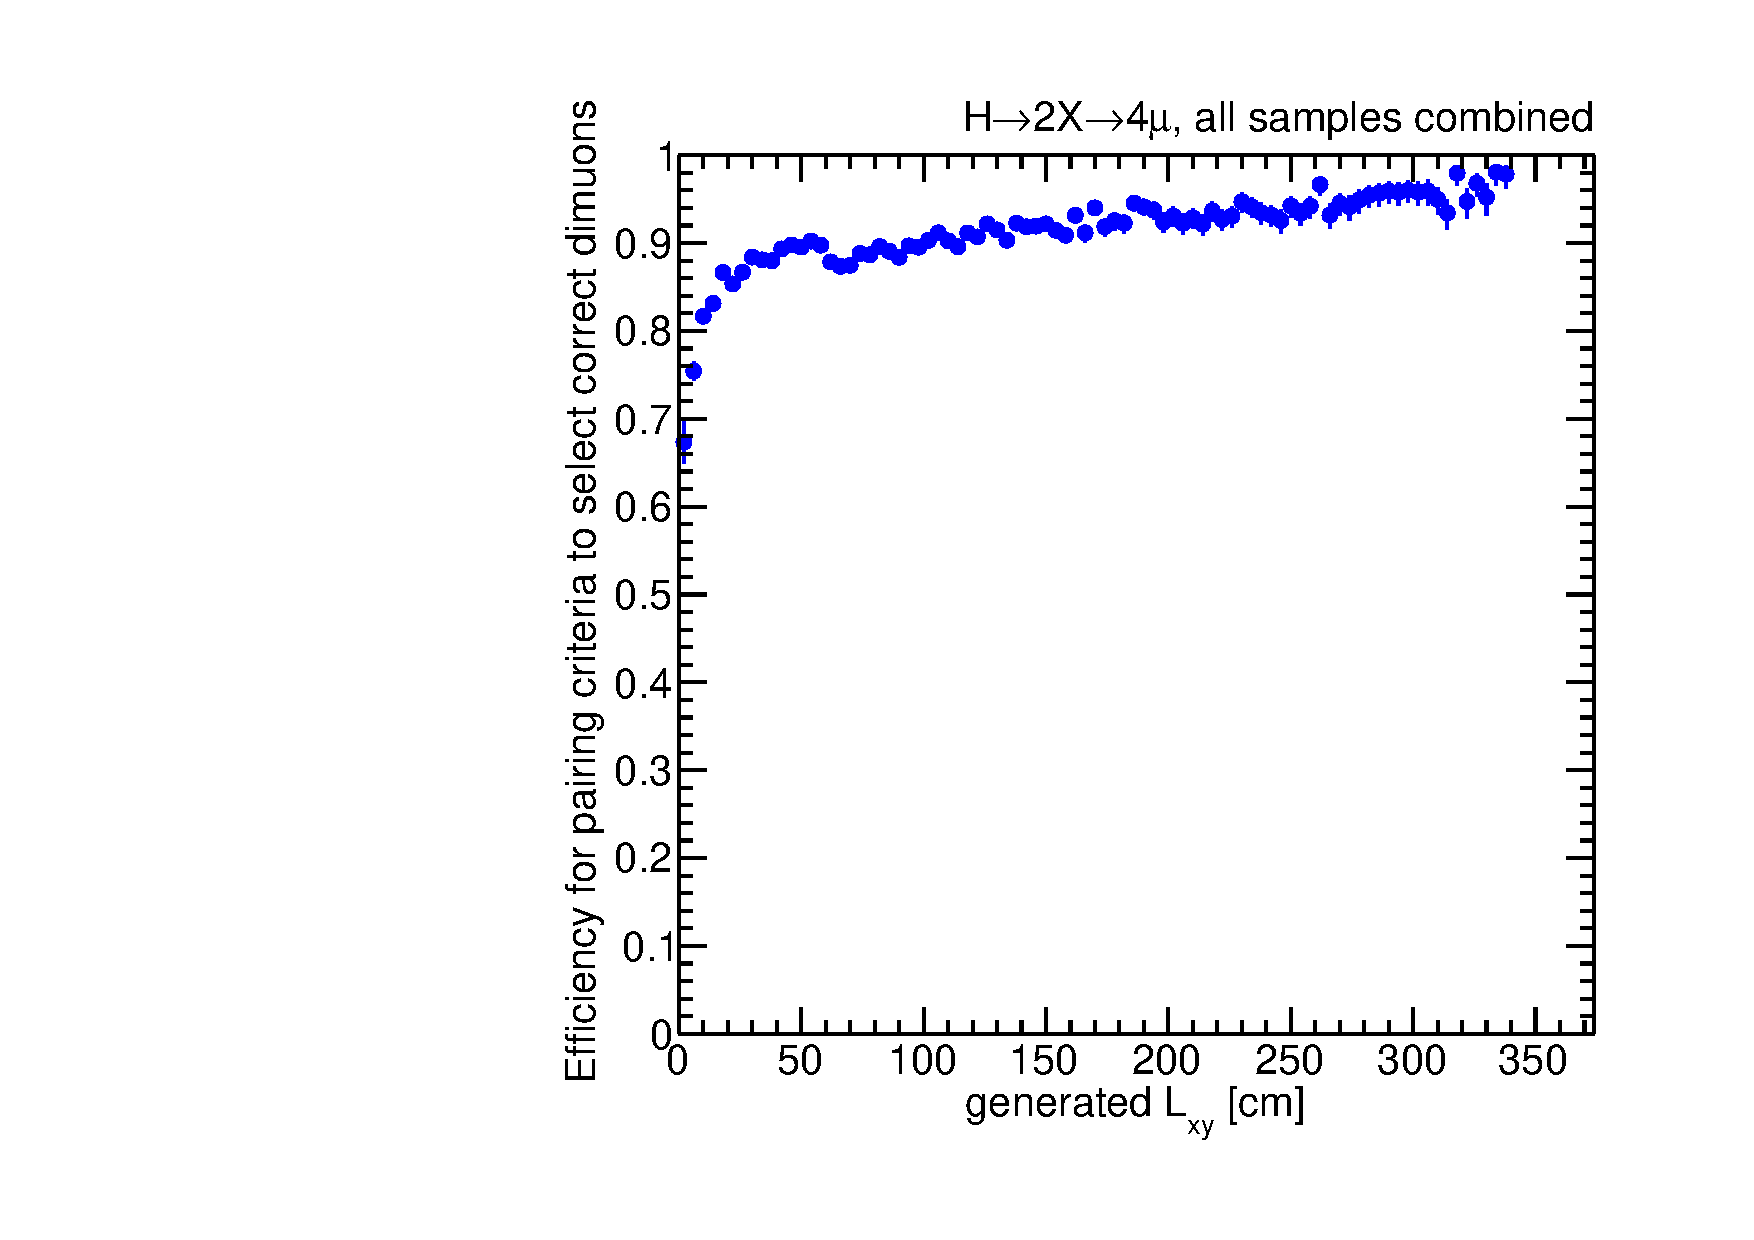
\includegraphics[width=\DSquareWidth]{figures/displaced/PC_Lxy_4Mu_Global.pdf}
  \caption{Efficiency for the pairing criteria to correctly choose reconstructed dimuons, as in \Fig~\ref{fig:dd:PC_Eff}, for all samples combined.}
  \label{fig:dd:PC_Eff_Global}
\end{figure}

\subsection{Dimuon Object Selection}
\label{sec:dd:DimuonObject}
Along with the DCA requirement, the requirement of convergence of the common vertex fit, and the application of the pairing criteria explained in \Sec~\ref{sec:dd:PC}, the following requirements serve as a dimuon identification selection.
These requirements further select high-quality dimuons as well as suppress background events.
Dimuons are required
\begin{itemize}
  \item to have a reconstructed dimuon mass of at least 10\GeV, \ie $\mMuMu > 10\GeV$
  \item to have a $\chi^2$ of the common vertex fit of at most 20, \ie $\chi^2_\text{vertex} < 20$
\end{itemize}

The \vchisq cut ensures that the dimuon is formed from tracks that can be reasonably well associated to a common vertex.
The mass cut suppresses complex backgrounds arising from QCD processes and events with low \pT and collimated muons.

\subsection{Dimuon Signal Selection}
\label{sec:dd:DimuonSignal}
The following criteria select displaced dimuons consistent with the signal hypothesis, \ie that the dimuon was constructed from two muons with opposite-sign ocharge that originated from the decay of a long-lived particle produced promptly, and therefore resulted in a dimuon vertex displaced from the beamspot.
The relevant quantities were defined in \Sec~\ref{sec:dd:keyvars}.
Dimuons are required
\begin{itemize}
  \item to have an \Lxy significance of at least 5, \ie $\Lxy/\LxyErr > 5$
  \item to have a transverse collinearity angle of less than $\pi/2$, \ie $|\DeltaPhi| < \pi/2$
  \item to be formed from two DSA muons with electric charges of opposite sign
\end{itemize}

\subsection{Cosmic Muon Suppression}
\label{sec:dd:CosmicCuts}
As mentioned in \Sec~\ref{sec:dd:VertexFitting}, one result of the common vertex fit of two muons is a pair of vertex-constrained tracks.
After the common vertex fit, a population of selected dimuons with relatively small \vchisq values was observed in data, and not in simulation, with the following unusual properties:
\begin{itemize}
  \item Muon vertex-constrained momentum $\phi$ directions changed by approximately $\pi$
  \item Muon vertex-constrained \pT uncertainties were unusually small, \ie $\pTErr/\pT \approx 10^{-7}\text{--}10^{-5}$
\end{itemize}
The presence of these dimuons were found to correlate with
\begin{itemize}
  \item Muons with relatively large transverse impact parameters, \ie $d_0 \approx 200\text{--}1000\cm$, and
  \item Events with no \pp collision vertices, and/or
  \item Events with large numbers of DSA muons, \ie $N(\text{DSA}) \approx 15\text{--}20$
    \begin{itemize}
      \item And these large numbers of DSA muons are largely parallel, \ie $|\cos{\alpha}| \approx 1$
    \end{itemize}
\end{itemize}
Further investigation suggested that these events are consistent with showers of cosmic muons.
\Fig~\ref{fig:dd:shower} is an example display of an event in data consistent with a shower of cosmic muons in a \pp collision event, containing a large number of approximately parallel pairs of DSA muons in addition to two global muons (not selected) originating from the \pp collision.

\begin{figure}[htpb]
  \centering
  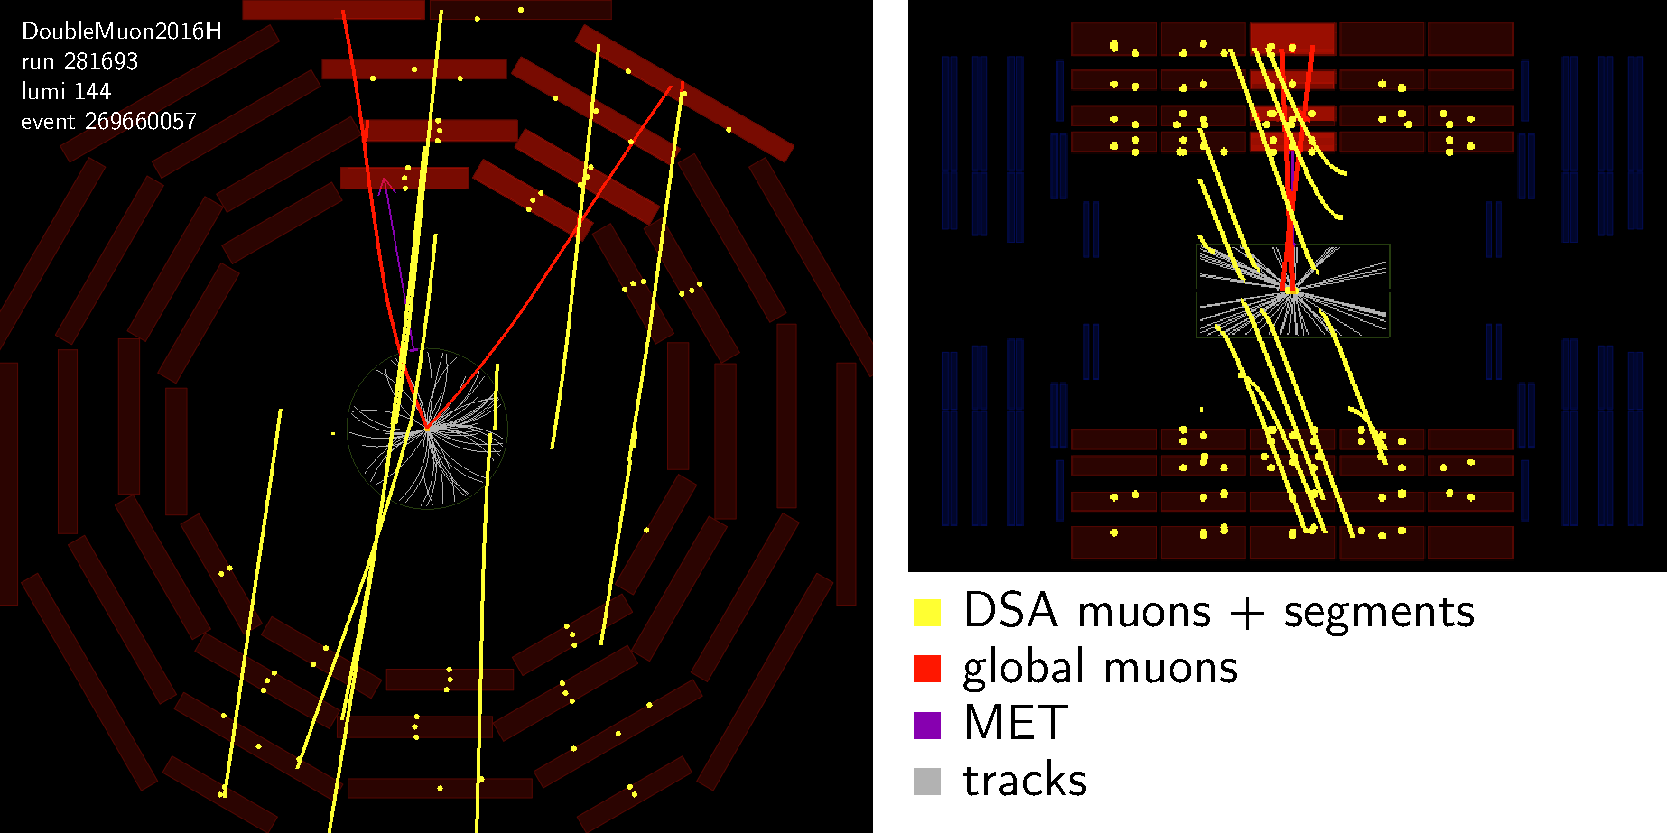
\includegraphics[width=\textwidth]{figures/displaced/ED_Cosmic.pdf}
  \caption{Display of an event in data consistent with a shower of cosmic muons in a \pp collision event. Two of the many approximately parallel DSA muons (yellow) reconstructed in this event formed a dimuon vertex with a good \vchisq and the event subsequently passed all our other selections. Requirements that events not contain too many parallel pairs of DSA muons and that the opening angle between the two muons not be too close to $\pi$ were found to be effective in suppressing such events.}
  \label{fig:dd:shower}
\end{figure}

A cosmic muon is often reconstructed as two back-to-back muons, one in the upper half of the detector and one in the lower half of the detector.
A reconstructed dimuon could also be formed from half a cosmic muon and a track from the \pp collision.
These dimuons are reconstructed as highly displaced, which is why the muons have such large $d_0$ values.
The common vertex fit was previously discussed to have anomalous behavior at large displacements, so the presence of the flip-by-$\pi$ and small \pT uncertainty anomalies when fitting to muons with large $d_0$ is perhaps not unexpected.
Such events are background events and so the analysis imposes a set of selections designed to suppress showers of cosmic muons.

Some of these events have no \pp collision vertices and contain only cosmic muons.
Events are therefore required to contain at least one well-identified vertex with position $(x, y, z)$ satisfying the following requirements:
\begin{itemize}
  \item At least 4 degrees of freedom when constructing the vertex
  \item $|z| < 24\mm$
  \item $\sqrt{x^2 + y^2} < 2\mm$
\end{itemize}
This set of requirements is referred to in CMS as the \Code{PrimaryVertexFilter}.

A typical strategy to suppress back-to-back cosmic muons is with a selection on $\cos{\alpha}$, and indeed the trigger has just such a cut, roughly equivalent to $\cos{\alpha} > -0.8$.
Following the trigger, our offline analysis selection also requires $\cos{\alpha} > -0.8$, on the opening angles both between the vertex-constrained muons and between the original (before the vertex fit) muons.

However, these two requirements alone are not sufficient to suppress all events consistent with cosmic muon showers.
As an additional measure to suppress cosmic muon showers, the analysis rejects events with a large number of parallel pairs of DSA muons.
All possible pairs of DSA muons, with no common vertex fit, are considered, and the number $N(\text{parallel pairs})$ of such pairs with $|\cos{\alpha}| > 0.99$ are counted.
The analysis selection then requires that events contain no more than 5 such pairs, verified to be of negligible efficiency in signal.

In summary, the cosmic muon suppression selections are
\begin{itemize}
  \item Events pass the \Code{PrimaryVertexFilter}
  \item Events have $N(\text{parallel pairs}) < 6$
  \item Dimuons have original and vertex-constrained $\cos{\alpha} > -0.8$
\end{itemize}

\subsection{Summary of Event and Object Selection}
\Tab~\ref{tab:dd:fullsel} summarizes the full event and object selections discussed in this section.
\begin{table}
  \centering
  \begin{tabular}{llll} 
    \hline\hline
    \multicolumn{4}{c}{Event Selection} \\
    \hline
    primary vertex                    & \multicolumn{3}{l}{\Code{PrimaryVertexFilter} passed}       \\
    HLT-RECO matching                 & \multicolumn{3}{l}{HLT-RECO matching algorithm found match} \\
    number of parallel DSA muon pairs & $N$(parallel pairs) & $<$ & 6                               \\
    \hline
    & & \\

    \hline\hline
    \multicolumn{4}{c}{DSA Muon Selection} \\
    \hline
    association with PAT muons         & \multicolumn{3}{l}{DSA muons \emph{not} associated to PAT muons}  \\
    number of CSC and DT stations      & $N$(CSC+DT stations)                      & $>$ & 1               \\
    number of CSC and DT hits          & $N$(CSC+DT hits)                          & $>$ & 12              \\
    number of DT hits for barrel muons & $N(\text{DT hits}\,\vert\,\text{barrel})$ & $>$ & 18              \\
    relative \pT uncertainty           & $\pTErr/\pT$                              & $<$ & 1               \\
    transverse muon momentum           & \pT                                       & $>$ & 10\GeV          \\
    normalized track \normchisq        & $\chisq_\text{track}/\text{dof}$          & $<$ & 4               \\
    \hline
    & & \\

    \hline\hline
    \multicolumn{4}{c}{Dimuon Selection} \\
    \hline
    distance of closest approach of muon & DCA                            & $<$ & 50\cm          \\
    common vertex fit                    & \multicolumn{3}{l}{common vertex fit converged}       \\
    pairing criteria                     & \multicolumn{3}{l}{best 1--2 ranked dimuons selected} \\
    dimuon mass                          & $\mMuMu$                       & $>$ & 10\GeV         \\
    vertex \chisq                        & $\chisq_\text{vertex}$         & $<$ & 20             \\
    cosine of dimuon 3D opening angle    & $\cos{\alpha}$                 & $>$ & $-0.8$         \\
    \Lxy significance                    & $\Lxy/\LxyErr$                 & $>$ & 5              \\
    transverse collinearity angle        & $|\DeltaPhi|$                  & $<$ & $\pi/2$        \\
    opposite sign muons                  & \multicolumn{3}{l}{constituent muons are oppositely charged} \\
    \hline
  \end{tabular}
  \caption{Summary of full selection, organized into event, muon, and dimuon requirements.}
  \label{tab:dd:fullsel}
\end{table}
